\documentclass[a4paper,12pt]{article}

\usepackage{fontspec}
\newfontfamily{\defaultfont}{CMU Serif}
\newfontfamily{\thaifont}[Scale=MatchLowercase]{TH Sarabun Chula}

\usepackage{polyglossia}
\setdefaultlanguage{thai}
\setotherlanguages{english}

\usepackage[Latin,Thai]{ucharclasses}
\setDefaultTransitions{\defaultfont}{}
\setTransitionTo{Thai}{\thaifont}

\XeTeXlinebreaklocale "th"
\XeTeXlinebreakskip = 0pt plus 0pt

\linespread{1.25}

\usepackage{amsmath,amsthm,amssymb}
\usepackage[ISO]{diffcoeff}
\usepackage{siunitx}
\usepackage[margin=1in]{geometry}
\usepackage{graphicx}
\usepackage{hyperref}
\usepackage{fancyhdr}
\pagestyle{fancy}
\rhead{Ittipat}
\lhead{ฟิสิกส์วิชาสามัญปี 2564}
\begin{document}
	\begin{titlepage}
	{\Huge{
			\vspace*{\fill}
			\noindent
			\makebox[\textwidth]
			{\title*{ข้อสอบฟิสิกส์วิชาสามัญปี 2564}}}
		\\\\
		{\Large{
				\makebox[\textwidth]
				{\title*{ขอขอบคุณข้อสอบจาก Tonsonphysics}}}
			\\\\	
		}}
	\vfill
	\end{titlepage}
	\begin{enumerate}
		\item นักเรียนคนหนึ่งต้องการวัดความยาวของวัตถุชิ้นหนึ่ง ซึ่งมีความยาวประมาณ 8 เซนติเมตร ด้วยไม้บรรทัดที่มีการแบ่งช่องสเกลที่มีความละเอียด 0.1 เซนติเมตร ทำการวัดความยาว 5 ครั้ง ได้ความยาวในหน่วย cm ดังนี้
		\begin{center}
			7.85 8.00 7.25 7.9 14.15
		\end{center}
		นักเรียนต้องการรายงานผลการวัดความยาวของวัตถุด้วยค่าเฉลี่ย \((\bar{x})\) 			และรายงานความคลาดเคลื่อนของค่าเฉลี่ย \((\bar{x})\) ด้วยสูตร
		\[\Delta \bar{x}=\frac{x_{\text{max}}-x_\text{min}}{2}\]
		เมื่อ \(x_{\text{max}}\) และ \(x_{\text{min}}\) คือค่าที่มากที่สุดและน้อยที่สุดที่วัดได้ตามลำดับ ข้อใดแสดงผลรายงานการวัดความยาวได้ถูกต้อง\\
		1. \(8\pm0.2\,\si{cm}\)\\
		2. \(8.0\pm0.2\,\si{cm}\)\\
		3. \(8.00\pm0.2\,\si{cm}\)\\
		4. \(9.2\pm3.2\,\si{cm}\)\\
		5. \(9.23\pm3.15\,\si{cm}\)
		\item คนขับรถคนหนึ่งกำลังขับรถด้วยความเร็วเนื่องจากมีกล้องตรวจจับอยู่ข้างหน้า จึงตัดสินใจชะลอความเร็วที่เวลา \(t=\SI{4.0}{s}\) โดยชะลอรถด้วยความเร่ง \(\SI{-0.5}{m/s^2}\) จนกระทั่งผ่านกล้องตรวจจับเวลาที่ \(t=\SI{34.0}{s}\) กำหนดให้กฎจราจรจำกัดความเร็วในการขับรถไม่เกิน \(\SI{120}{km/h}\) หรือ \(\SI{33.3}{m/s}\) ถ้าทำผิดกฎจราจรจะต้องเสียค่าปรับ ได้กราฟแสดงอัตราเร็วของรถกับเวลาดังนี้
		\begin{figure}[h]
			\centering
			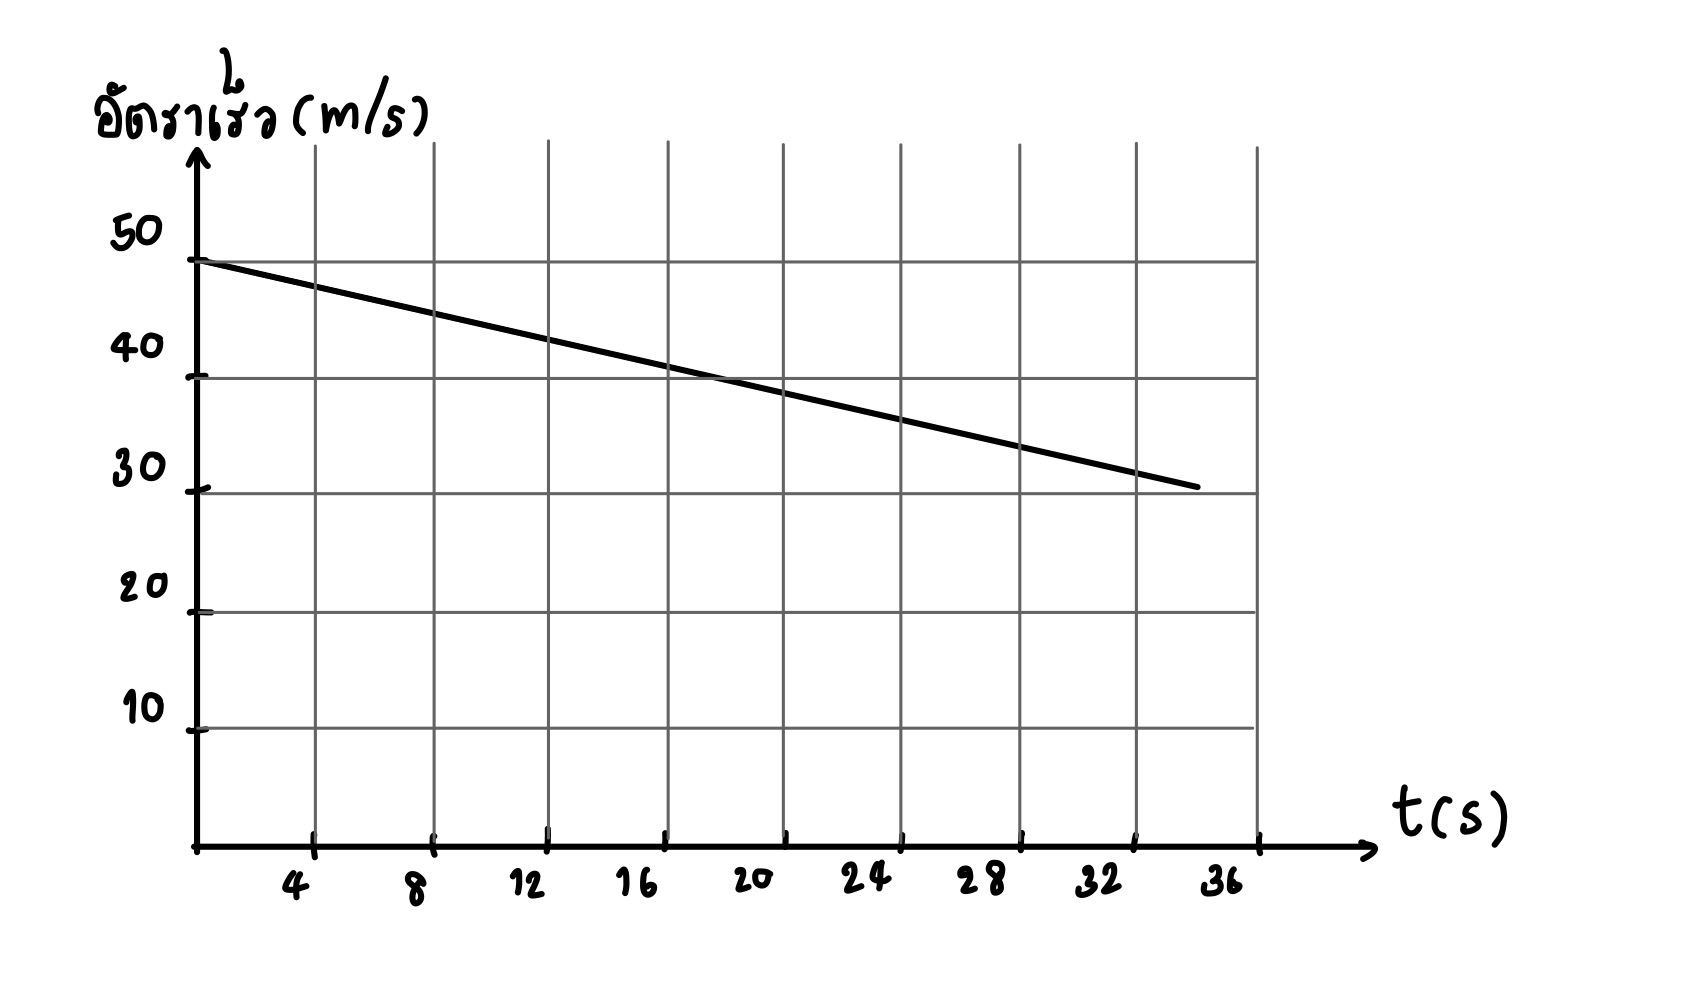
\includegraphics[width=0.7\linewidth]{2}
		\end{figure}
		
		กราฟนี้สอดคล้องกับสถาณการณ์ของโจทย์หรือไม่และคนขับรถต้องเสียค่าปรับหรือไม่
			\vspace{4cm}
		
		\item วัตถุมวล \(\SI{0.5}{kg}\) มีแรงสามแรงมากระทำดังภาพ
		\begin{figure}[h]
			\centering
			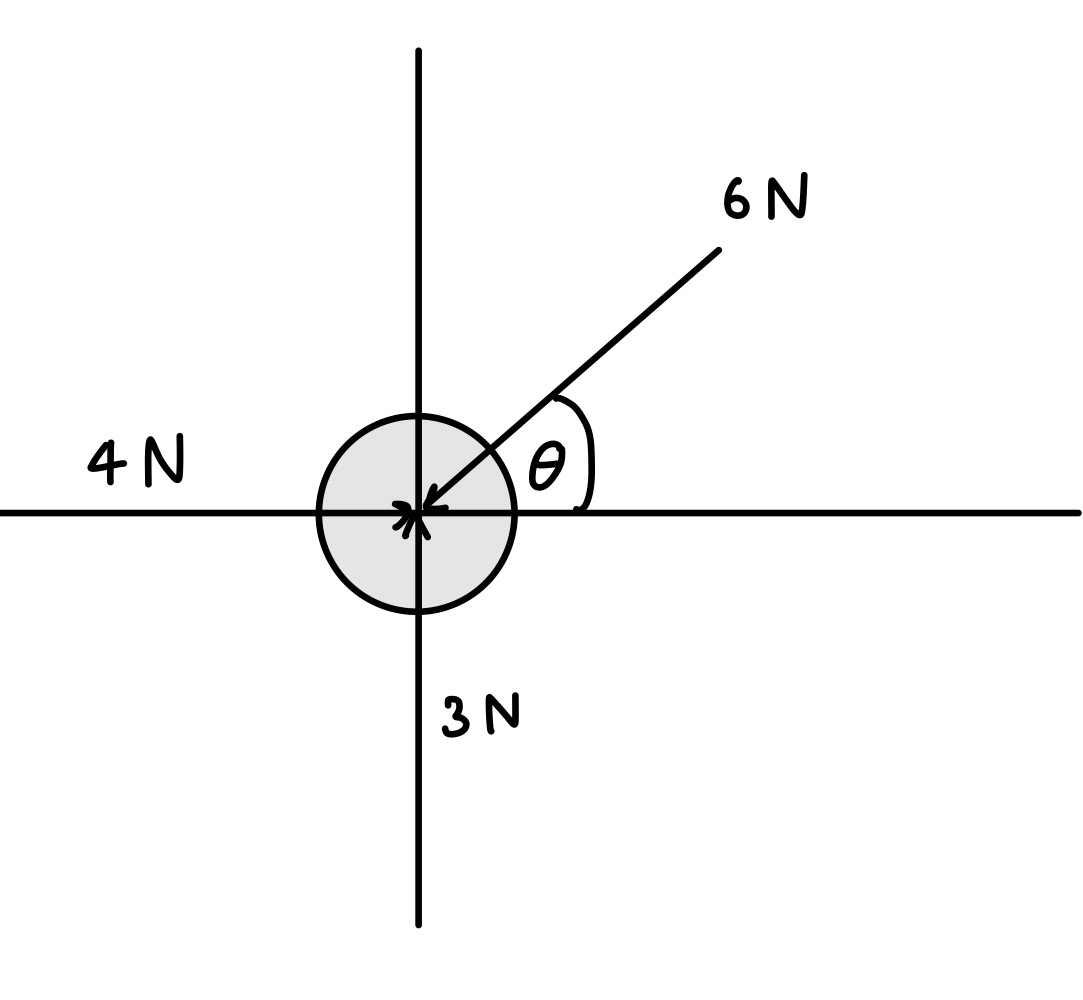
\includegraphics[width=0.3\linewidth]{3}
		\end{figure}\\
		จงแสดงขนาดและทิศทางของความเร่งของวัตถุ (กำหนดให้ \(\sin\theta=\frac{3}{5}\) และ \(\cos\theta=\frac{4}{5}\))
			\vspace{4cm}
		
		\item ยกวัตถุมวล \(\SI{1.0}{kg}\) ขึ้นไปจากพื้นจากหยุดนิ่งด้วยแรงคงที่ค่าหนึ่ง เมื่อผ่านไป \(\sqrt{10}\,\si{s}\) ระบบมีพลังงานศักย์โน้มถ่วงเท่ากับ \(\SI{98}{J}\) เทียบกับพื้น จงหาขนาดของแรงที่ใช้ดึงวัตถุขึ้น
			\vspace{4cm}
		
		\item นาย A และนาย B ต้องการแบกคานสม่ำเสมอยาว \(\SI{3}{m}\) หนัก \(\SI{50}{N}\) ซึ่งมีกล่องหนัก \(\SI{150}{N}\) แขวนไว้ที่จุดห่างจากจุดกึ่งกลางเป็นระยะ \(\SI{0.2}{m}\) ไปทางนาย A โดยที่นาย A และ B แบกคานที่จุดที่ห่างจากปลายคาน \(\SI{0.5}{m}\) ดังภาพ
		\begin{figure}[h]
			\centering
			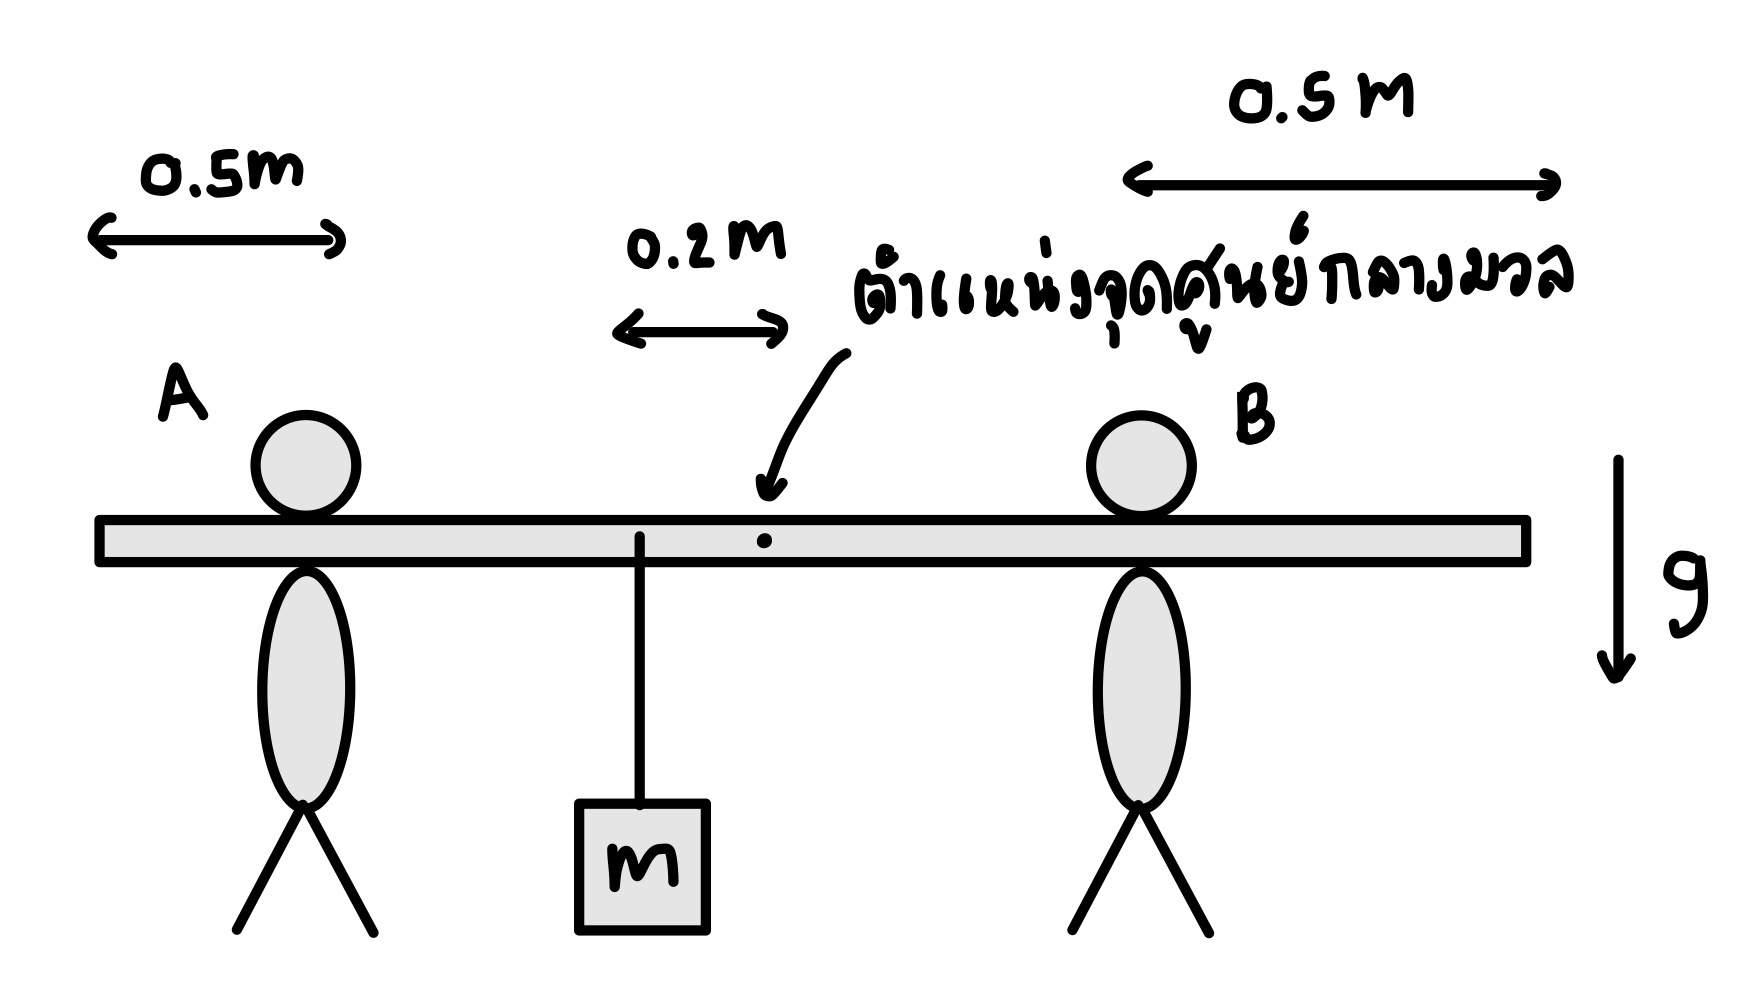
\includegraphics[width=0.5\linewidth]{5}
		\end{figure}\\
		ถ้าต้องการให้นาย A และ B แบกคานด้วยแรงที่เท่ากันและนาย B แบกคานที่ตำแหน่งเดิม ถามว่านาย A จะต้องขยับตัวเข้าหาหรือออกจากกล่องเป็นระยะเท่าใด
			\vspace{4cm}
		
		\item กำหนดระบบรอกซึ่งแขวนมวลหนัก \(W\) ไว้ดังรูป
		\begin{figure}[h]
			\centering
			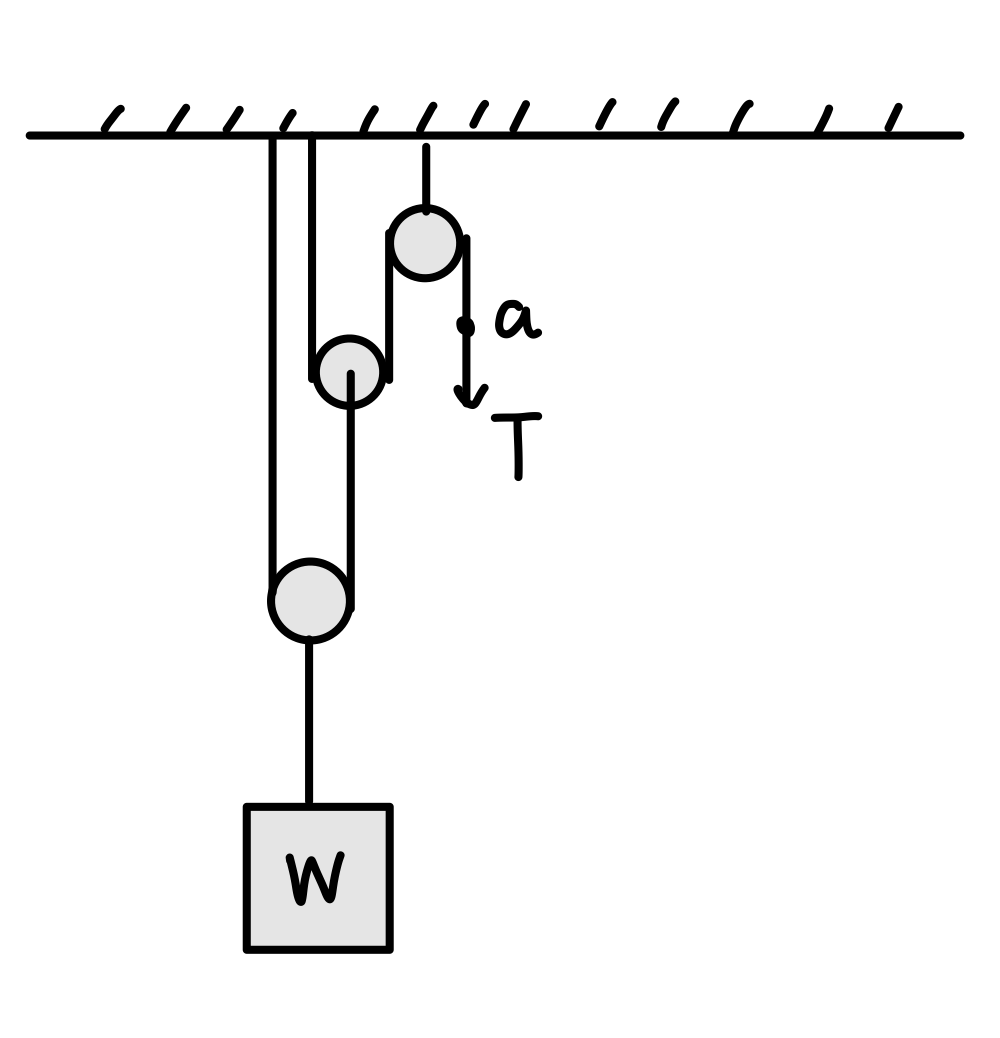
\includegraphics[width=0.3\linewidth]{6}
		\end{figure}\\
	ถ้าต้องการดึกปลายเชือกที่จุด a ด้วยแรง \(T\) ลงไปเป็นระยะ \(D\) ทำให้ยกวัตถุหนัก \(W\) ขึ้นได้พอดี จงหาความสัมพันธ์ของ \(T\) ในรูปของ \(W\) และวัตถุจะยกขึ้นไปได้เป็นระยะทางเท่าใด
			\vspace{4cm}
		
		\item ถ้าดาวเทียม A มวล \(m\) โคจรรอบโลกโดยรัศมี \(R_\text{A}\) และอัตราเร็ว \(v_\text{A}\) ดังภาพ
		\begin{figure}[h]
			\centering
			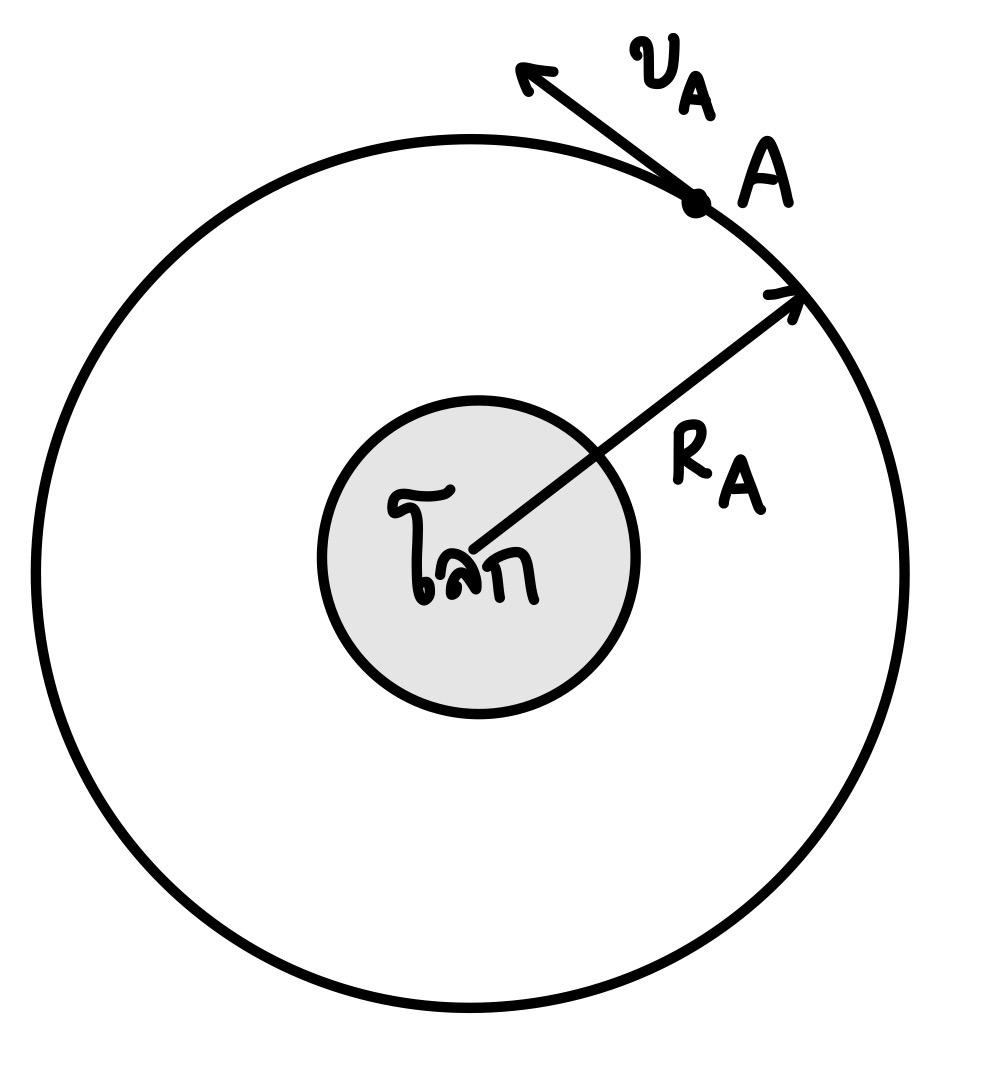
\includegraphics[width=0.3\linewidth]{7}
		\end{figure}\\
	ถ้าต้องการส่งดาวเทียม B ที่มีมวล \(2m\) ให้โคจรด้วยรัศมี \(R_\text{B}\) และอัตราเร็ว \(v_\text{B}\) จงเปรีบเทียบ \(R_\text{B},v_\text{B}\) เทียบกับ \(R_\text{A},v_\text{A}\) (มากกว่า, น้อยกว่า, เท่ากัน\textenglish{)}
			\vspace{4cm}
		
		\item เมื่อวัตถุมวล \(M\) ติดด้วยสปริงและทำให้สั่นแบบ SHM ตามภาพ ก พบว่าเวลาที่ทำให้วัตถุเคลื่อนที่ครบหนึ่งรอบเท่ากับ \(\sqrt{2}\,\si{s}\) แต่ถ้านำวัตถุมวล \(\SI{1}{kg}\) วางซ้อนไว้ด้านบนตามภาพ ข พบว่าเวลาที่ทำให้วัตถุเคลื่อนที่ครบหนึ่งรอบเท่ากับ \(\sqrt{3}\,\si{s}\) 
		\begin{figure}[h]
			\centering
			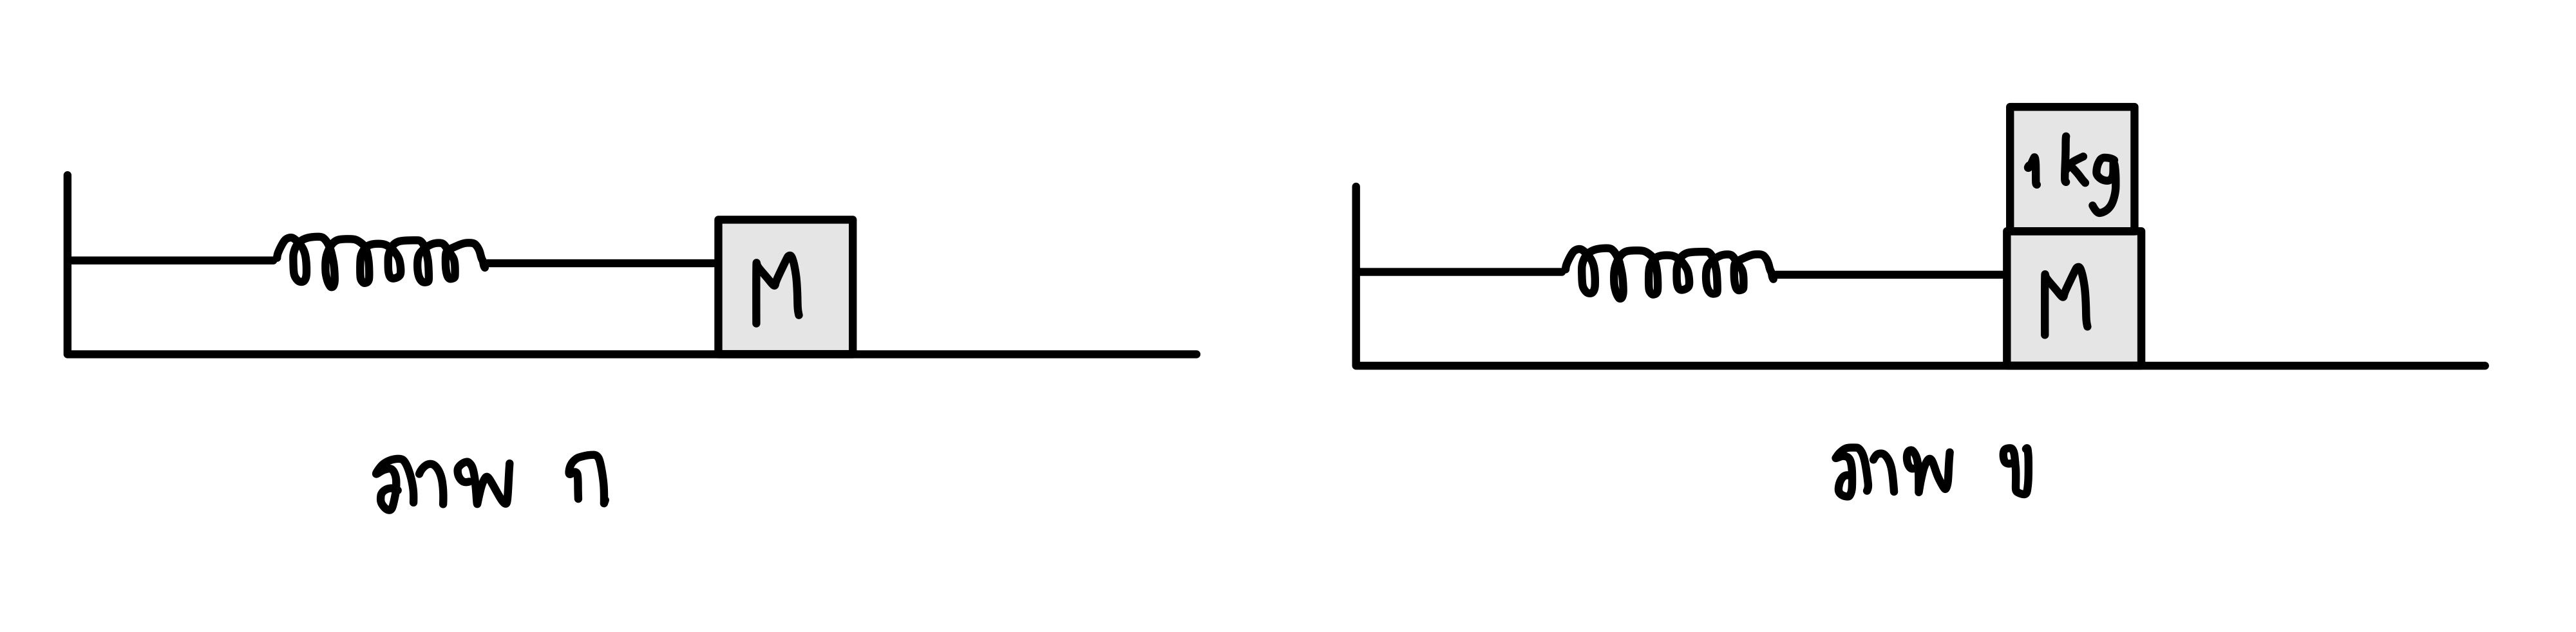
\includegraphics[width=0.9\linewidth]{8}
		\end{figure}
	จงหาความถี่เชิงมุมในการสั่นของรูป ก และขนาดของมวล \(M\)
			\vspace{4cm}
		
		\item พิจารณาคลื่นสองขบวนที่กำลังเคลื่อนที่เข้าหากันที่เวลา \(t=\SI{0.0}{s}\) ด้วยอัตราเร็ว \(\SI{1.0}{m/s}\)
			\begin{figure}[h]
			\centering
			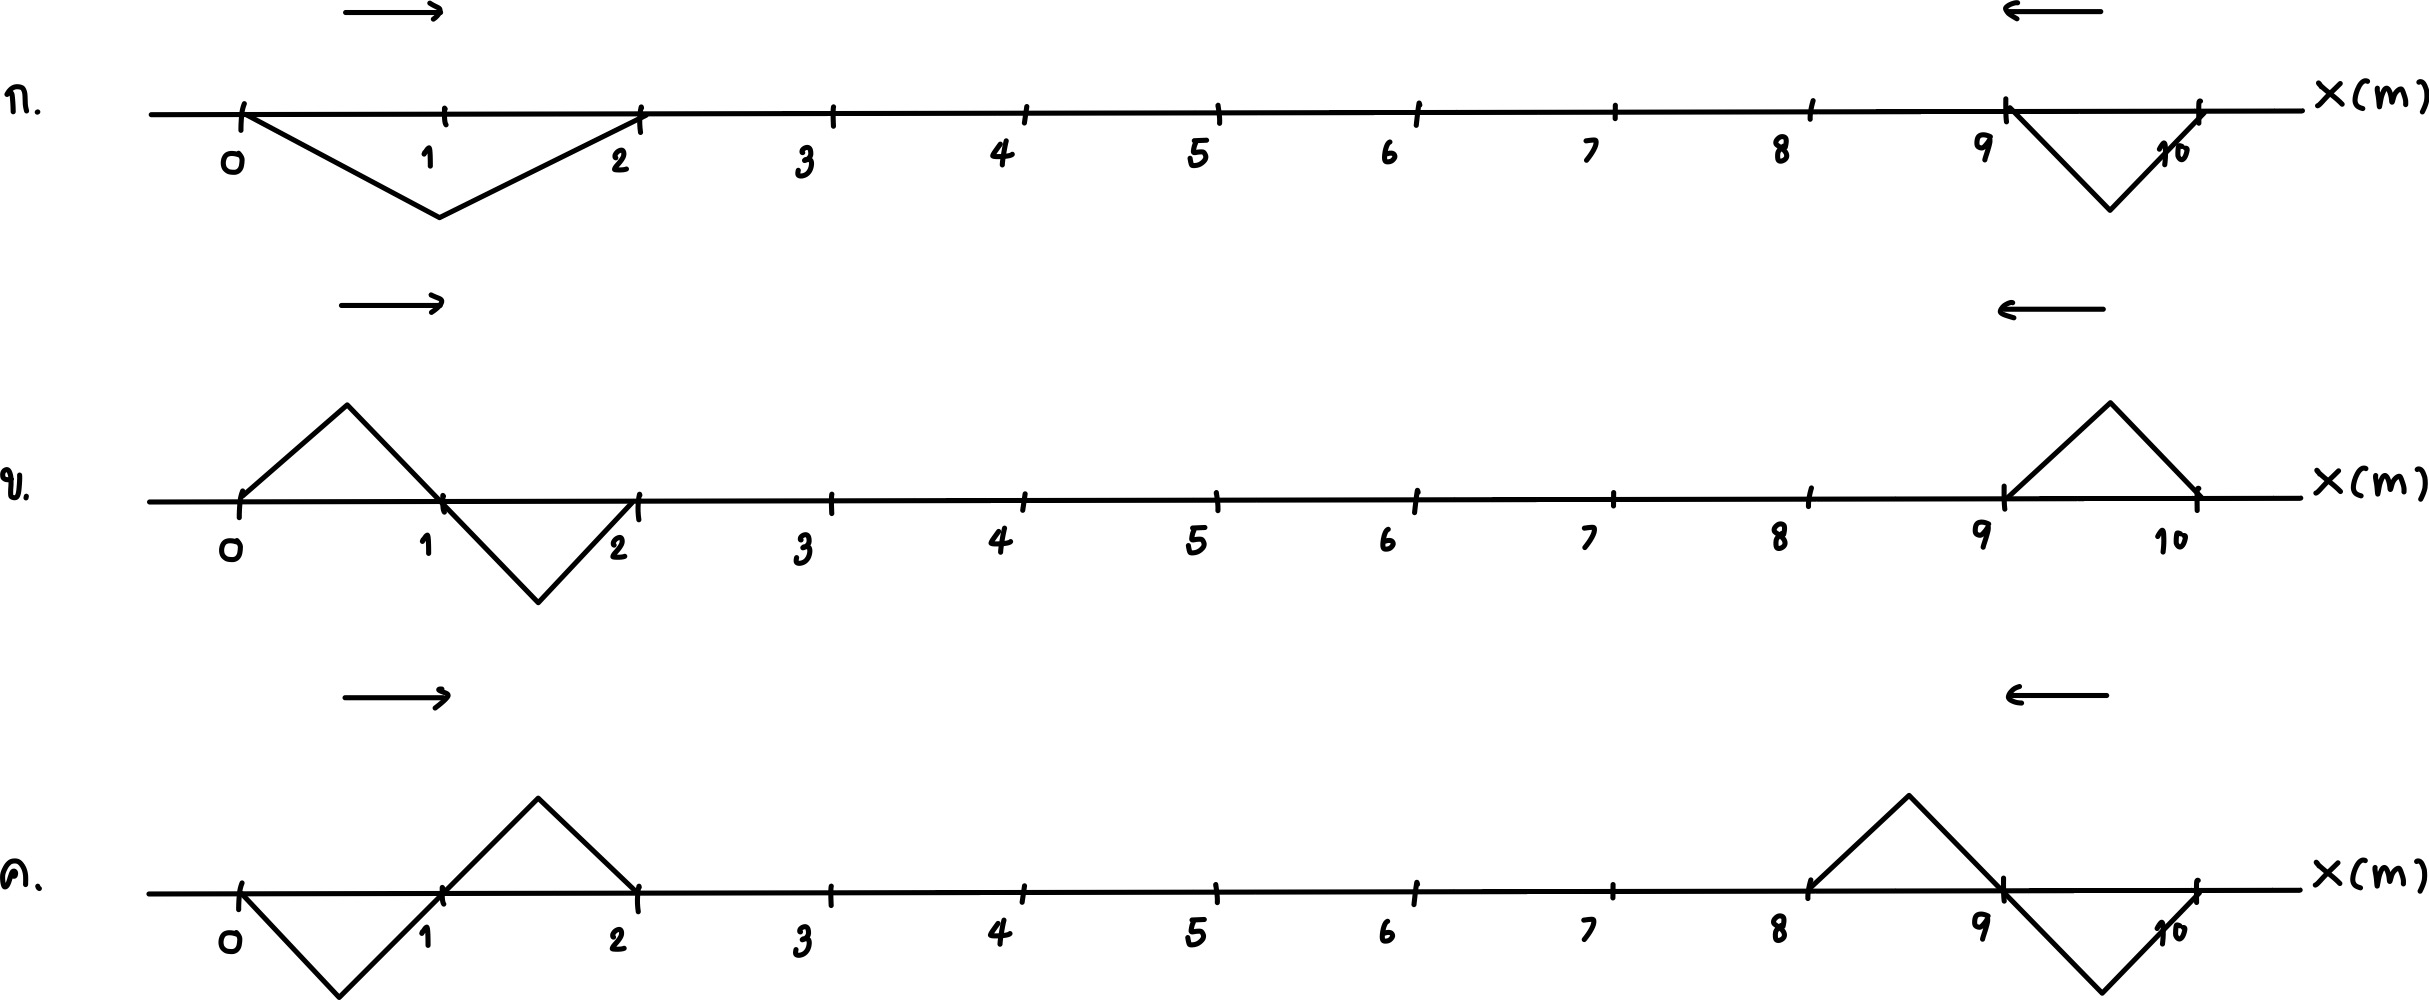
\includegraphics[width=0.7\linewidth]{9}
		\end{figure}\\
		สถาณการณ์ใดบ้างที่เกิดการแทรกสอดแบบหักล้างที่เวลา \(t=\SI{4.0}{s}\)
			\vspace{4cm}
		
		\item นาย A และนาย B ยืนอยู่ห่างกันเป็นระยะ \(\SI{100}{m}\) ถ้านาย A เป่านกหวีด ทำให้นาย B ได้ยินเสียงนกหวีดด้วยระดับเสียง \(\SI{30}{dB}\) จงหากำลังเสียงที่เกิดจากนาย A เป่านกหวีด
			\vspace{4cm}
		
		\item ทำการทดลองสลิตคู่ที่มีระยะระหว่างสลิต \SI{0.05}{mm} เมื่อฉายเแสงผ่านสลิต จึงพบริ้วรอยแถบมือแถบสว่างบนฉาก จากนั้นเปลี่ยนจากสลิตคู่เป็นสลิตเดี่ยว แล้วฉายแสงความยาวคลื่นเดิมผ่านสลิต พบว่าตำแหน่งของแถบมือลำดับแรกของสลิตเดี่ยว เป็นตำแหน่งเดียวกับแถบมืดลำดับแรกของสลิตคู่ จงหาความกว้างของสลิตเดี่ยว
			\vspace{4cm}
		
		\item นักเรียนคนหนึ่งกำลังมองวัตถุผ่านกล้องที่ประกอบจากเลนส์นูน 2 ชิ้นที่อยู่ห่างกัน \(\SI{18}{cm}\) พบว่าภาพที่เกิดจากการหักเหครั้งแรก เกิดที่ระยะ \(\SI{15}{cm}\) ห่างจากเลนส์ 1 ดังภาพ 
		\begin{figure}[h]
			\centering
			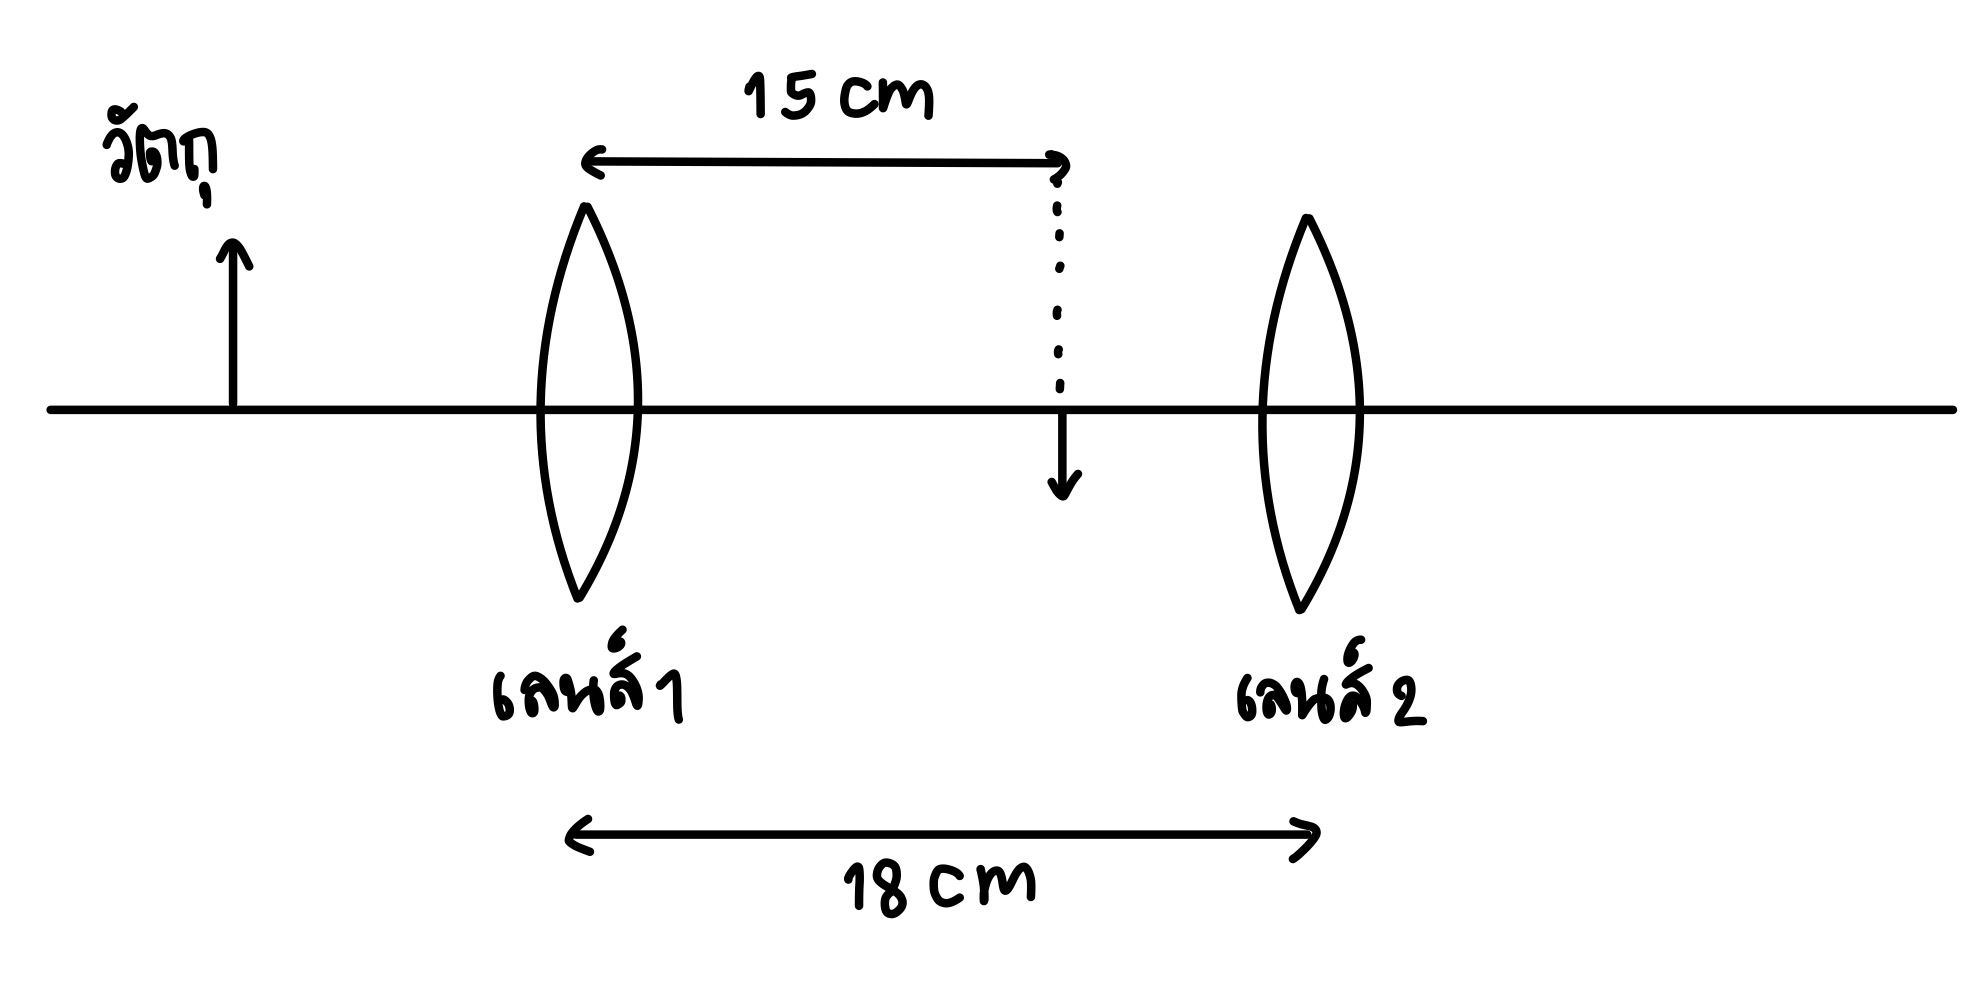
\includegraphics[width=0.7\linewidth]{12}
		\end{figure}\\
	ถ้าต้องการเห็นภาพเสมือนที่มีขนาดเป็น 2 เท่าของภาพจากกการหักเหครั้งแรกเลนส์ 2 จะต้องมีความยาวโฟกัสเท่าไร
			\vspace{4cm}
		
		\item กำหนดประจุไฟฟ้าขนาด \(-q\) และ \(+2q\) วางอยู่ที่จุดยอดของสี่เหลี่ยมจัตุรัสที่มีความยาวด้านละ \(d\) ดังภาพ
		\begin{figure}[h]
			\centering
			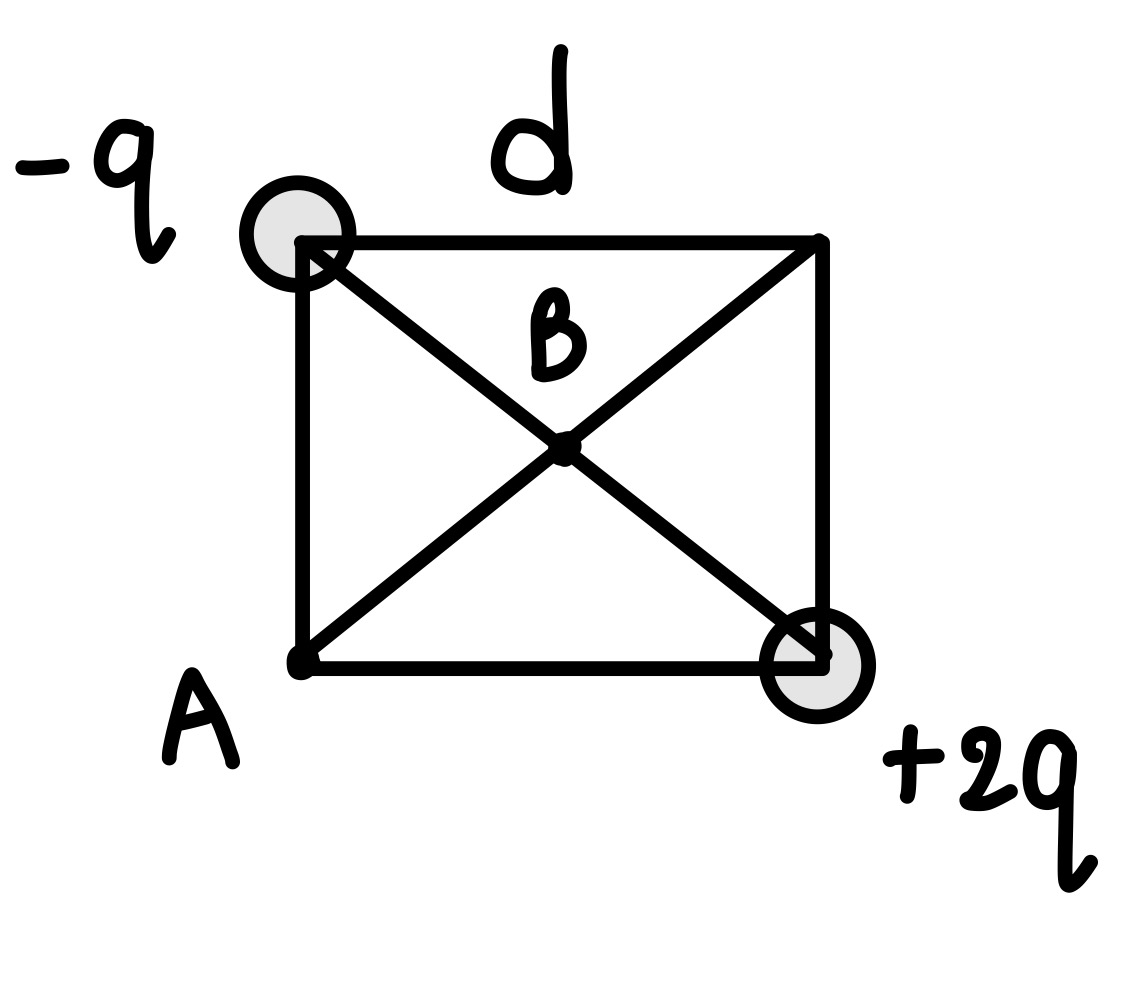
\includegraphics[width=0.3\linewidth]{13}
		\end{figure}
	จงหาความต่างศักย์ระหว่างจุด A และจุด B \((V_\text{A}-V_\text{B})\)
			\vspace{4cm}
		
		\item กำหนดวงจรตัวเก็บประจุที่มีตัวเก็บประจุ 2 ตัว คือ \(C\) และ \(2C\) ต่ออนุกรมกันเข้ากับแบตเตอรี่ขนาด \(\SI{6}{V}\) ดังภาพ
		\begin{figure}[h]
			\centering
			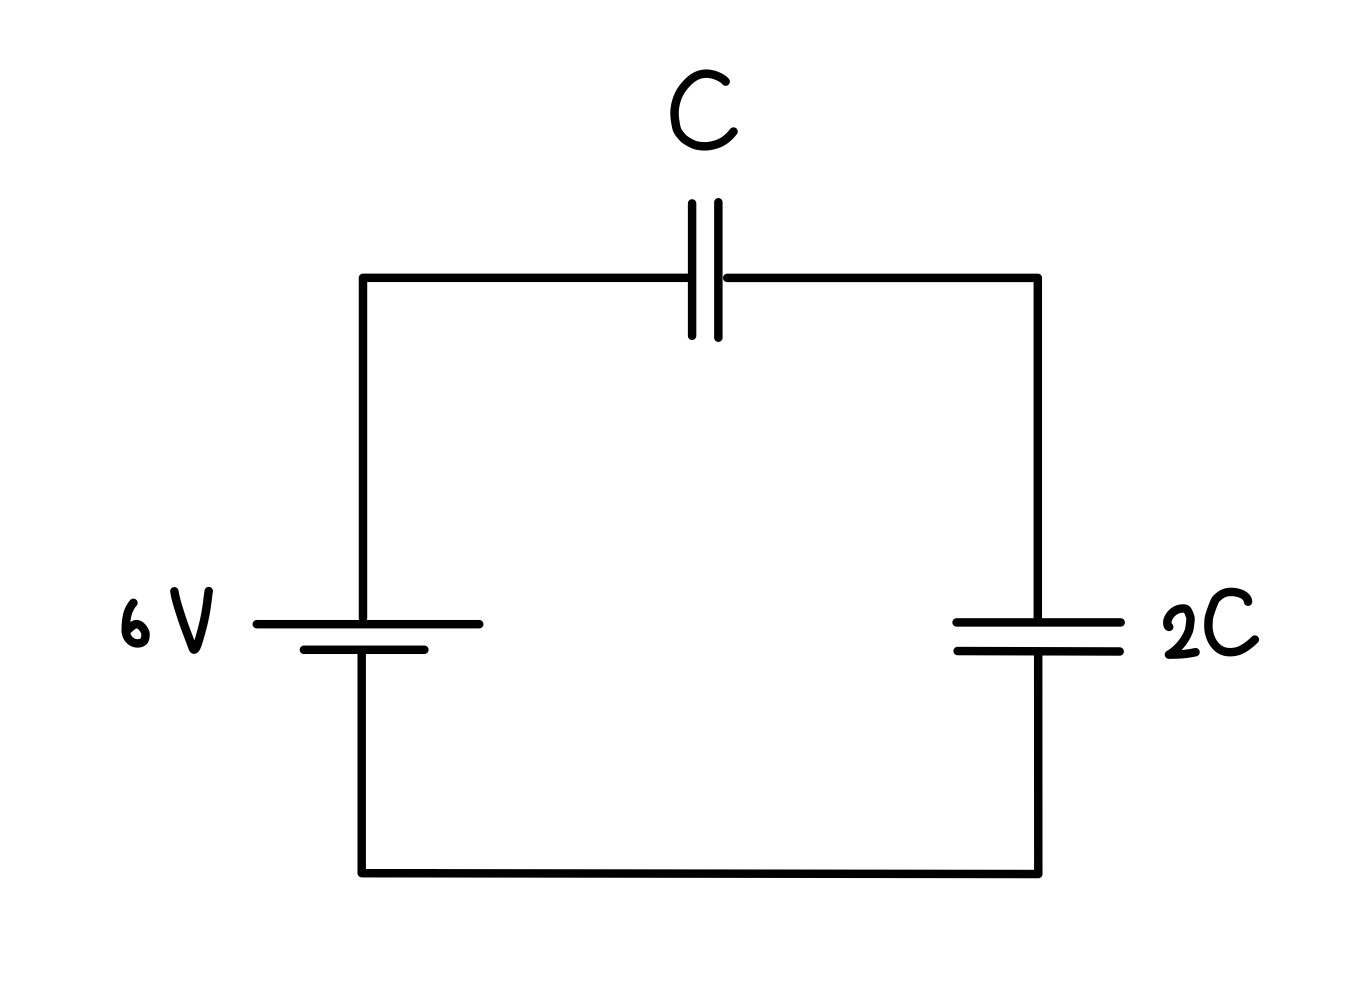
\includegraphics[width=0.3\linewidth]{14}
		\end{figure}
		ถ้า
		\begin{itemize}
			\item วงจรนี้มีค่าความสมมูลเท่ากับ \(\SI{4}{\micro F}\)
			\item ความต่างศักย์คร่อมตัวเก็บประจุ \(C\) เท่ากับ \(\SI{4}{V}\)
			\item ความต่างศักย์คร่อมตัวเก็บประจุ \(2C\) เท่ากับ \(\SI{2}{V}\) 
		\end{itemize}
		พลังงานที่สะสมในตัวเก็บประจุ \(2C\) มีค่าเท่ากับกี่ไมโครจูล
			\vspace{4cm}

		\item กำหนดอุปกรณ์ไฟฟ้าอันหนึ่งมีความต้านทาน \(\SI{40}{\ohm}\) ซึ่งจะทำงานได้เมื่อมีกระแสไฟฟ้าไหลผ่าน \(0.10\) ถึง \(0.15\) แอมแปร์ ถ้ามีวงจรไฟฟ้าที่นำอุปกรณ์ชิ้นนี้ต่อเข้ากับแบตเตอรี่ขนาด \(\SI{24}{V}\) และตัวต้านทาน \(\SI{100}{\ohm}\) ใน 3 ลักษณะ ดังภาพ
		\begin{figure}[h]
			\centering
			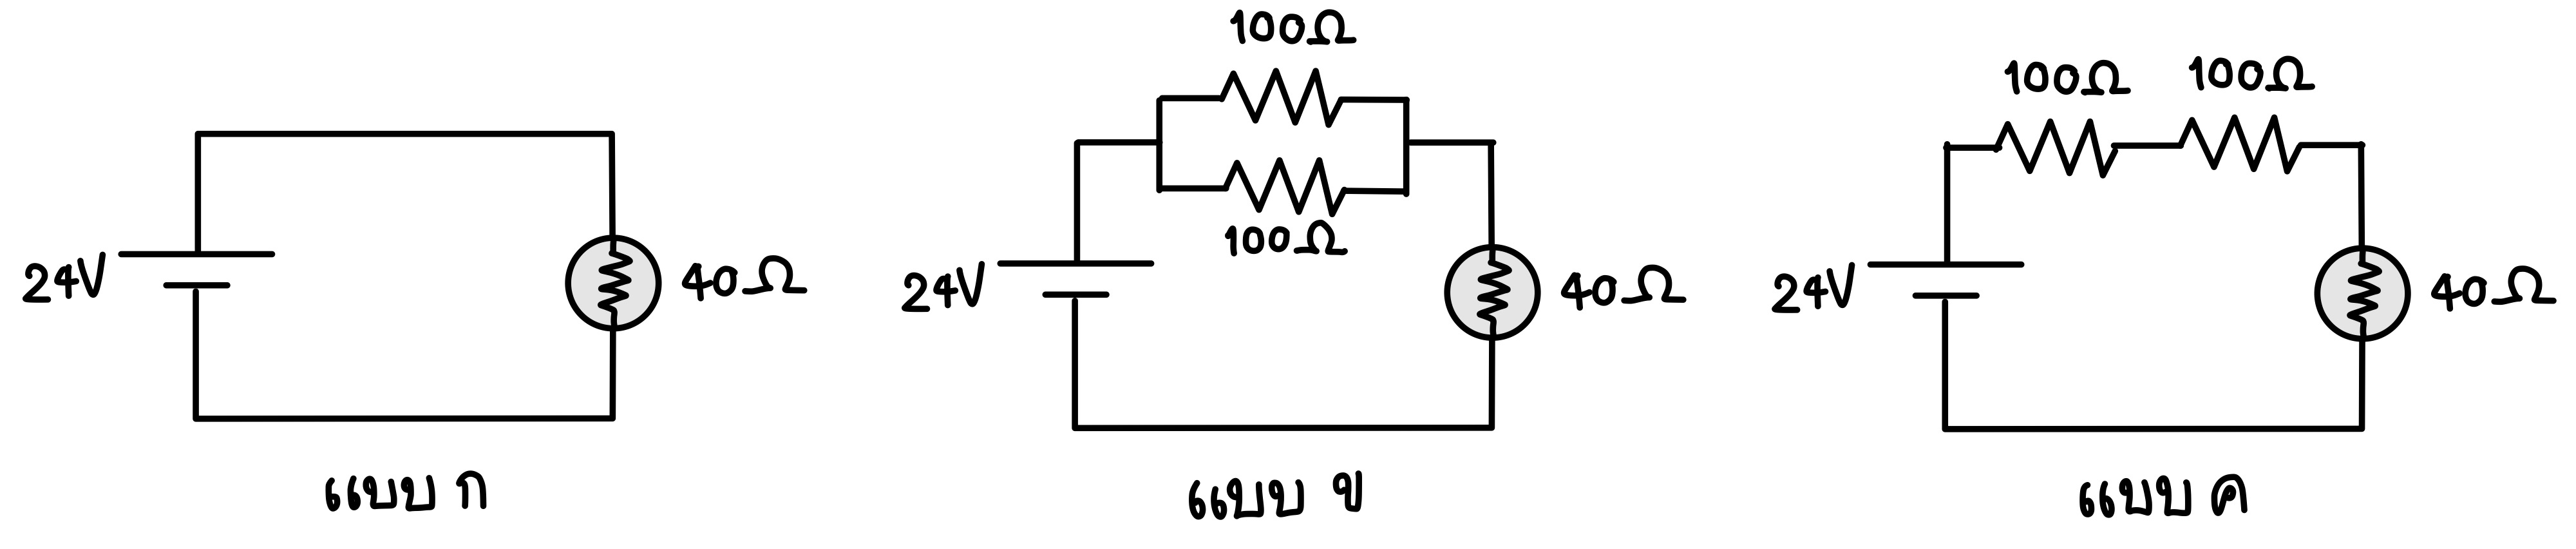
\includegraphics[width=0.8\linewidth]{15}
		\end{figure}
		วงจรแบบใดบ้างที่ทำให้อุปกรณ์ทำงานได้
			\vspace{4cm}
		
		\item ประจุไฟฟ้า A, B, C มีอัตราส่วนประจุต่อมวลเท่ากัน วิ่งเข้าไปในบริเวณที่มีสนามแม่เหล็กพุ่งเข้าไปในกระดาษ ได้เส้นทางการเคลื่อนที่ดังภาพ
		\begin{figure}[h]
			\centering
			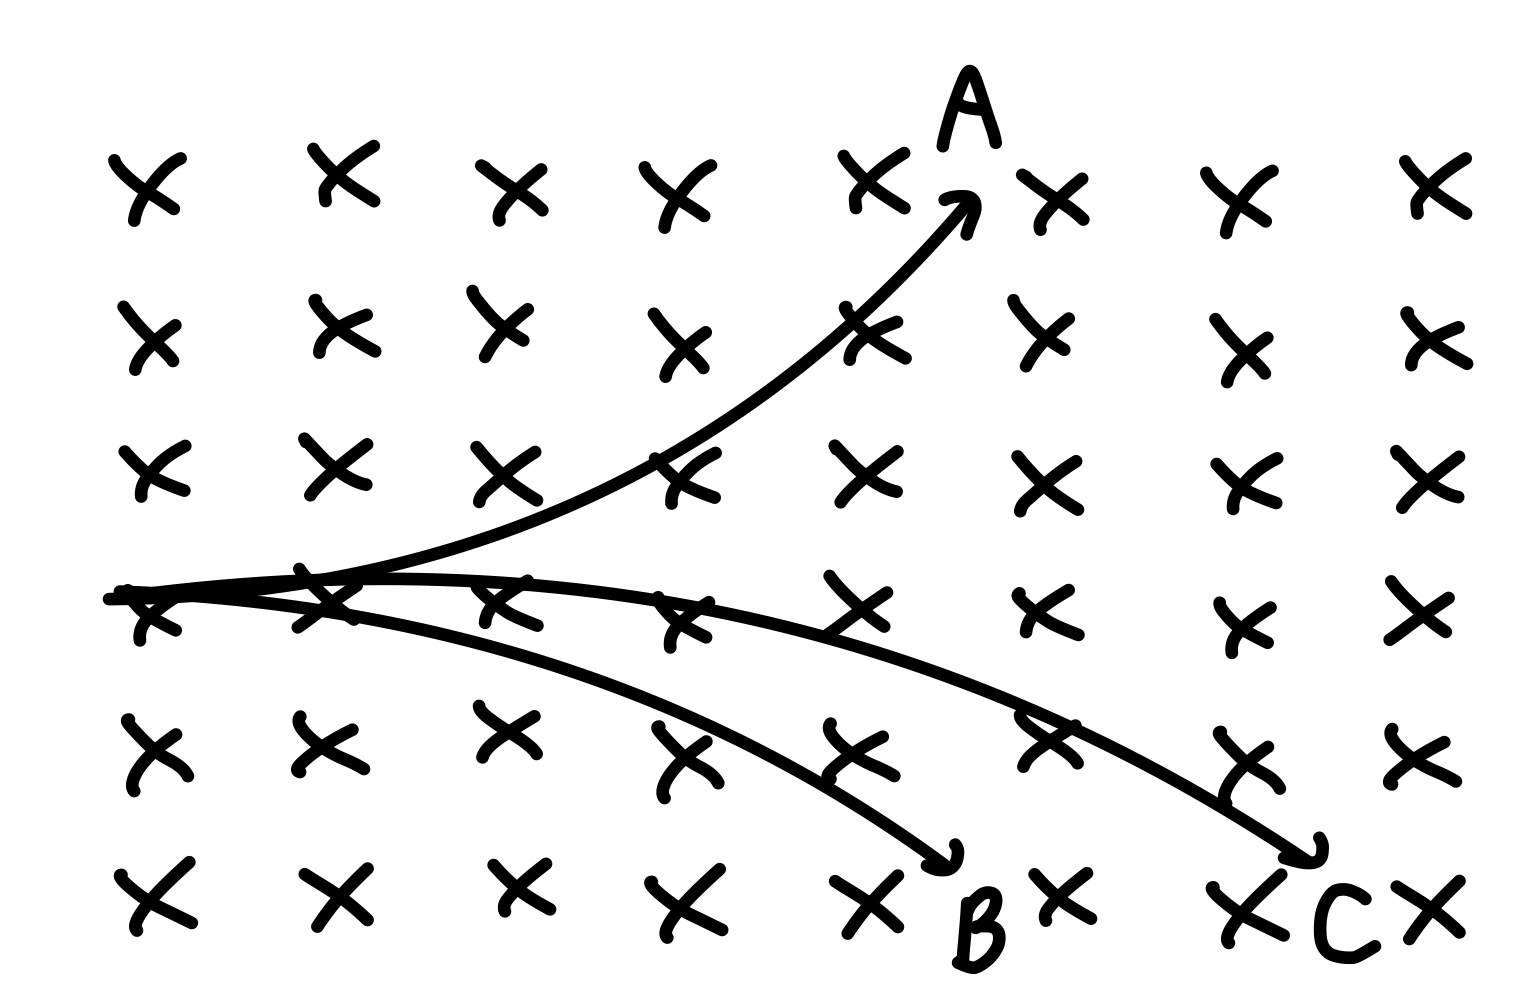
\includegraphics[width=0.3\linewidth]{16}
		\end{figure}\\
		ข้อใดต่อไปนี้ถูกต้อง\\
		1. อนุภาค A และ B เป็ยนประจุชนิดเดียวกัน\\
		2. อนุภาค B และ C เป็นประจุต่างชนิดกัน\\
		3. อนุภาค C เป็นประจุบวก\\
		4. อัตราเร็วของอนุภาค A มากกว่าของอนุภาค B\\
		5. อัตราเร็วของอนุภาค C มากกว่าของอนุภาค A\\
		
		\item จงพิจารณาความถูกผิดของข้อความต่อไปนี้\\
		(๑\textenglish{)} เครื่องรับวัทยุทำงานโดยการแปลงสัญญาณเสียงจากสถานีให้เป็นสัญญาณไฟฟ้า\\
		(๒\textenglish{)} คลื่นไมโครเวฟ เป็นคลื่นแม่เหล็กไฟฟ้าที่ใช้ในระบบ GPS\\
		(๓\textenglish{)} สัญญาณที่ใช้ในการสื่อสาร ที่มีการเปลี่ยนแปลงเพียง 2 ค่า คือ +1 และ -1 คือสัญญาณอนาลอก\\
		ข้อใดถูกต้อง\\
		1. ข เท่านั้น\\
		2. ค เท่านั้น\\
		3. ก และ ข\\
		4. ก และ ค\\
		5. ข และ ค
		\item วงจรไฟฟ้ากระแสสลับ ประกอบดว้ยตัวต้านทาน \(\SI{2}{\ohm}\) ต่อเข้ากับแหล่งกำเนิดไฟฟ้ากระแสสลับ ดังภาพ
		\begin{figure}[h]
			\centering
			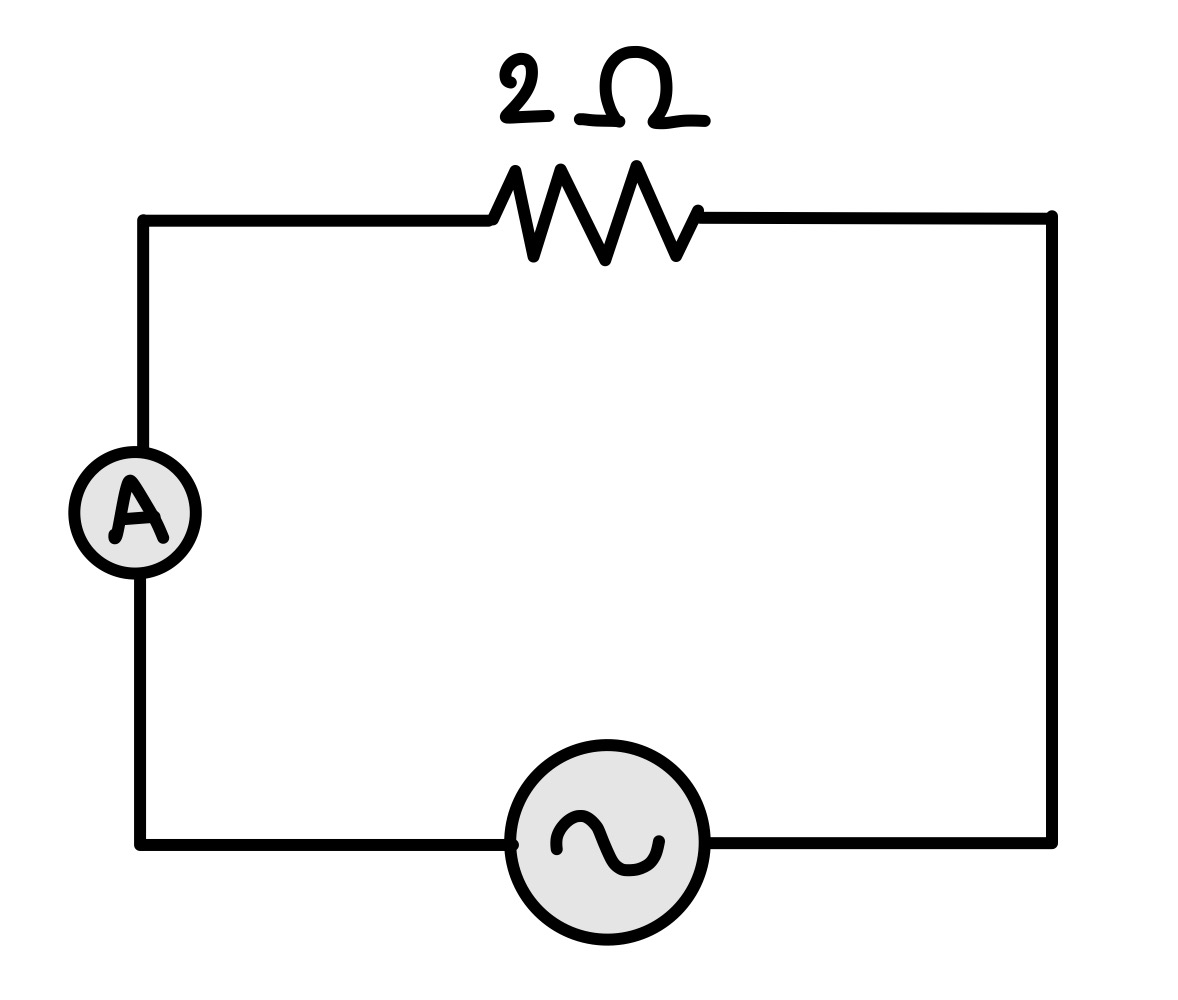
\includegraphics[width=0.3\linewidth]{18}
		\end{figure}\\
		ถ้าทำการวัดค่ายังผลของกระแสไฟฟ้าที่ไหลในวงจร พบว่ามีค่าเท่ากับ \(\SI{7.0}{A}\) ข้อใดแสดงกราฟแสดงความสัมพันธ์ระหว่างกระแสไฟฟ้า \((i)\) และความต่างศักย์ระหว่างปลายตัวต้านทาน \((v)\) ที่เปลี่ยนแปลงตามเวลาได้ถูกต้อง\\
		(กำหนดให้ \(\sqrt{2}=1.4,\frac{1}{\sqrt{2}}=0.7\))
			\vspace{4cm}	
			
		\item ของแข็ง A มวล \(\SI{1.0}{kg}\) มีอุณหภูมิตั้งต้น \(\SI{-10}{\degreeCelsius}\)\\
		ของเหลว B มวล \(\SI{2.0}{kg}\) มีอุณหภูมิตั้งต้น \(\SI{80}{\degreeCelsius}\)\\
		นำวัตถุ A และ B ไว้ด้วยกันในระบบปิด จนกระทั่งเข้าสู่สมดุลความร้อนที่เวลา \(t_\text{B}\) ได้กราฟการเปลี่ยนแปลงของอุณหภูมิของ A และ B ตามเวลาดังนี้
		\begin{figure}[h]
			\centering
			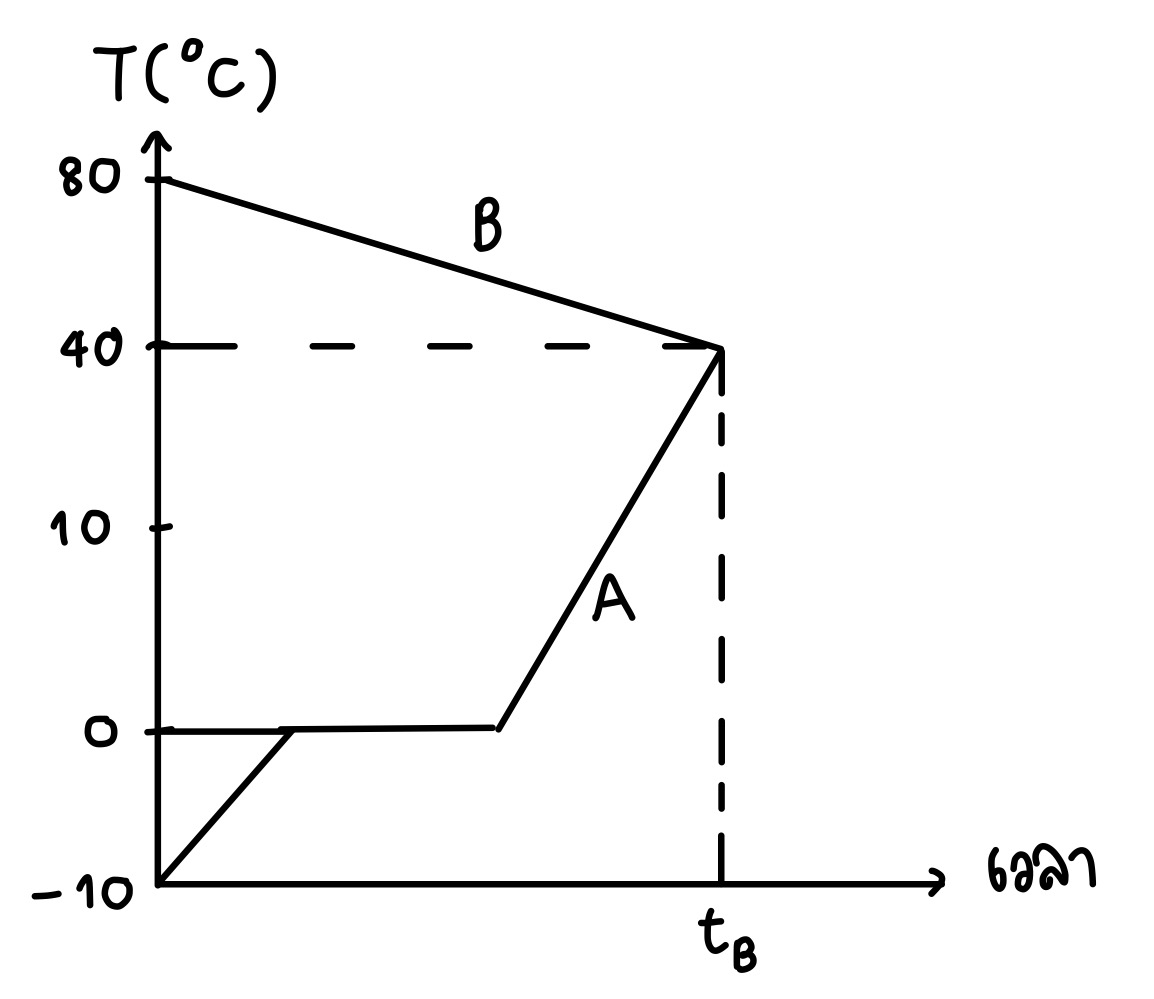
\includegraphics[width=0.3\linewidth]{19}
		\end{figure}
		กำหนดให้\\
		ความร้อนจำเพาะในสถานะของแข็งของ \(\text{A}=\SI{1.0e3}{J/kg\cdot K}\)\\
		ความร้อนแผงในการหลอมเหลวของ \(\text{A}=10^4\,\si{J/kg}\)\\
		ความร้อนจำเพาะในสถานะของเหลวของ \(\text{A}=\SI{2.0e3}{J/kg\cdot K}\)\\
		จงหาว่า ความร้อนจำเพาะในสถานะของเหลว B เท่ากับเท่าใดและหลังจากที่เวลา \(t_\text{B}\) ของเหลว B จะมีการเปลี่ยนแปลงอุณหภูมิอย่างไร (เพิ่มขึ้น, เท่าเดิม, ลดลง\textenglish{)}
			\vspace{4cm}
		
		\item แก๊ส He และ Ar ปริมาณเท่ากัน ถูกบรรจุในภาชนะเดียวกัน จนกระทั่งอยู่ในสภาวะสมดุลความร้อน จงพิจารณาความถูกผิดของข้อความต่อไปนี้\\
		(๑\textenglish{)} Ar มีพลังงานจลน์เฉลี่ยมากกว่า He\\
		(๒\textenglish{)} He มีอัตราเร็วเฉลี่ยมากกว่า Ar\\
		(๓\textenglish{)} Ar ทุกโมเลกุลมีอัตราเร็วเท่ากันหมด
			\vspace{4cm}
		
		\item ทำการทดลองเพื่อหาค่า Young modulus ของแท่งวัตถุอันหนึ่ง ซึ่งมีพื้นที่หน้าตัด \(A\) และความยาวตั้งต้น \(L_0\) โดยนำมวล \(m\) มาห้อยกับแท่งวัตถุที่ยึดกับเพดานได้ดังภาพ แล้วดูระยะยืด \(\Delta L\) ของแท่งโลหะโดยปรับค่า \(m\) หลายค่า จากนั้นนำข้อมูลที่ได้ไปพล็อตกราฟ \(\Delta L-m\) ได้กราฟเส้นตรงที่มีความชัน \(=k\)
		\begin{figure}[h]
			\centering
			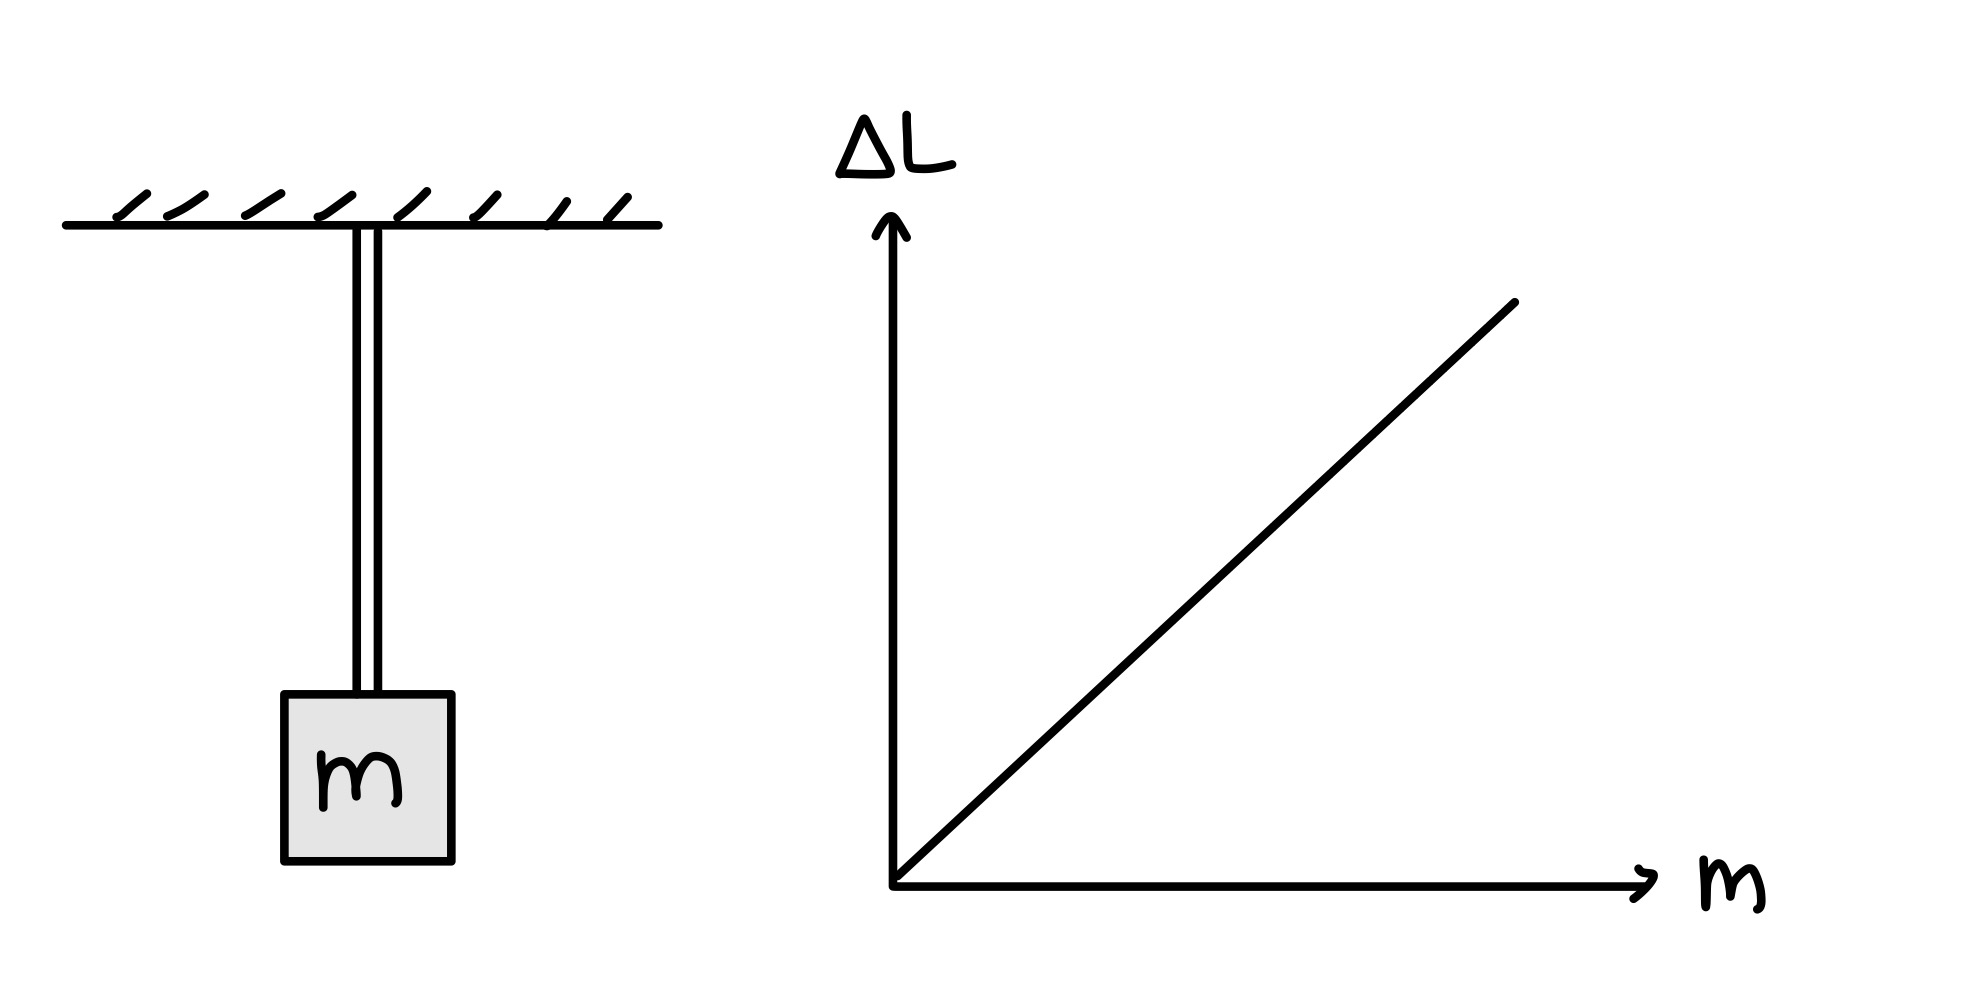
\includegraphics[width=0.5\linewidth]{21}
		\end{figure}
		ถ้าต้องการนำความชัน \(k\) ไปคำนวณเพื่อหาค่า Young modulus \(Y\) จงหาค่า \(Y\) ในรูปของค่าคงที่ในโจทย์
			\vspace{6cm}
		
		\item ท่อน้ำท่อหนึ่งมีน้ำความหนาแน่น \(\rho\) ไหลเข้าที่ความดันเป็น 10 เท่าของความดันบรรยากาศ \(P_0\) และไหลออกผ่านท่อที่เปิดสู่ความดันบรรยากาศ \(P_0\) ที่ความสูง \(H\) เหนือระดับขาเข้า ผ่านพื้นที่หน้าตัด \(\frac{1}{\sqrt{2}}\) เท่าของท่อขาเข้า 
		\begin{figure}[h]
			\centering
			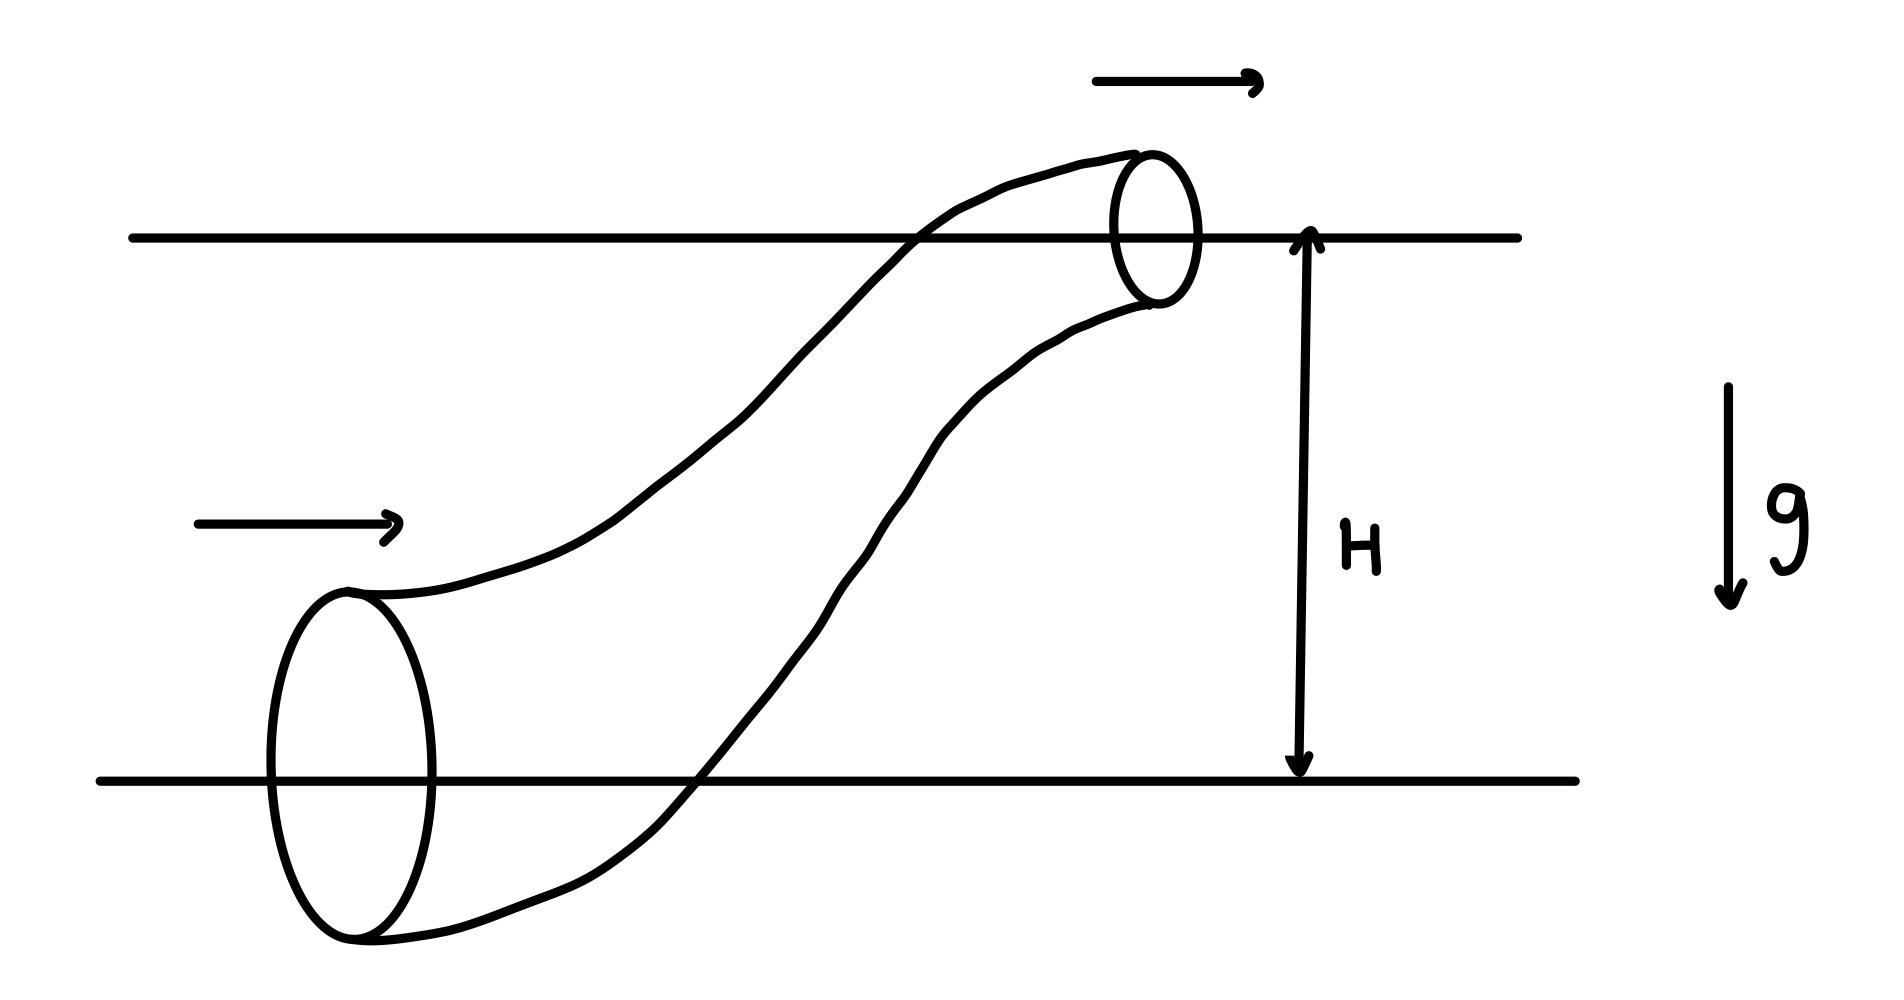
\includegraphics[width=0.5\linewidth]{22}
		\end{figure}จงหาอัตราเร็วของน้ำที่ไหลผ่านท่อขาออก
			\vspace{4cm}	
\newpage		
		\item กำหนดข้อมูลของอนุภาคมูลฐาน ดังนี้\\
		\begin{center}

		\begin{tabular}{|c|c|c|}
			\hline
			ชื่อ & มวล (\si{GeV/e^2}) & ประจุ (\si{e}) \\
			\hline
			down & 4.7 & -1/3 \\
			\hline
			up & 2.2 & 2/3 \\
			\hline
			strange & 96 & -1/3 \\
			\hline
			charm & 1.28 & 2/3 \\
			\hline
			bottom & 4.18 & -1/3 \\
			\hline
			top & 173.1 & 2/3 \\
			\hline
			electron & 0.51 & -1 \\
			\hline
			electron neutrino & <2.2 & 0 \\
			\hline
			muon & 105.66 & -1 \\
			\hline
			muon neutrino & <0.17 & 0 \\
			\hline
			tau & 1.78 & -1 \\
			\hline
			tau neutrino & <18.2 & 0 \\
			\hline
			photon & 0 & 0 \\
			\hline
			W & 80.39 & \(\pm1\) \\
			\hline
			Z & 91.19 & 0 \\
			\hline
			gluon & 0 & 0 \\
			\hline
		\end{tabular}
		\end{center}
		ถ้ามีอนุภาคหนึ่งซึ่งประกอบด้วย up quark และ strange antiquark อย่างละ  1 อนุภาค จงพิจารณาความถูกผิดของข้อความต่อไปนี้\\
		(๑\textenglish{)} อนุภาคนี้มีประจุเท่ากับ Z-boson\\
		(๒\textenglish{)} อนุภาคนี้มีมวลเท่ากับ Tau neutrino\\
		(๓\textenglish{)} อนุภาคนี้มี photon เป็นอนุภาคสื่อแรงที่เชื่อม quark เข้าด้วยกัน
			\vspace{4cm}
		
		\item อะตอมของไฮโดรเจนในสภาวะกระตุ้น มีการปลดปล่อยโฟตอนที่มีควอนตัมของพลังงาน \(\SI{1.89}{eV}\) จนอะตอมมีพลังงานรวม \(\SI{-3.4}{eV}\) จงหาอะตอม \(\text{H}_2\) มีการเปลี่ยนแปลงระดับพลังงานจากชั้นใดเป็นชั้นใด
			\vspace{4cm}
		
		\item ถ้านิวเคลียสของธาตุกัมมันตรังสีหนึ่งมีจำนวน \(\num{1.85e9}\) นิวเคลียสมีกัมมตภาพรังสี 1 มิลลิคูรี จงหาว่าต้องใช้เวลาเท่าใด นิวเคลียสของธาตุนี้จึงจะสลายตัวจนเหลือครึ่งหนึ่ง
		กำนหดให้ 1 คูรี \(=\num{3.7e10}\) วินาที\(^{-1}\)
			\vspace{4cm}
		
		\item ปืนใหญ่มวล \(\SI{400}{kg}\) อยู่บนพื้นฝืดที่มีสัมประสิทธิ์ความเสียดทานจลน์เท่ากับ \(0.5\) ยิงกระสุนมวล \(\SI{9.8}{kg}\) ออกไปด้วยอัตราเร็ว \(\SI{40}{m/s}\) จงหาว่าปืนใหญ่จพถอยหลังเป็นระยะกี่\underline{เซนติเมตร}\\
		\begin{figure}[h]
			\centering
			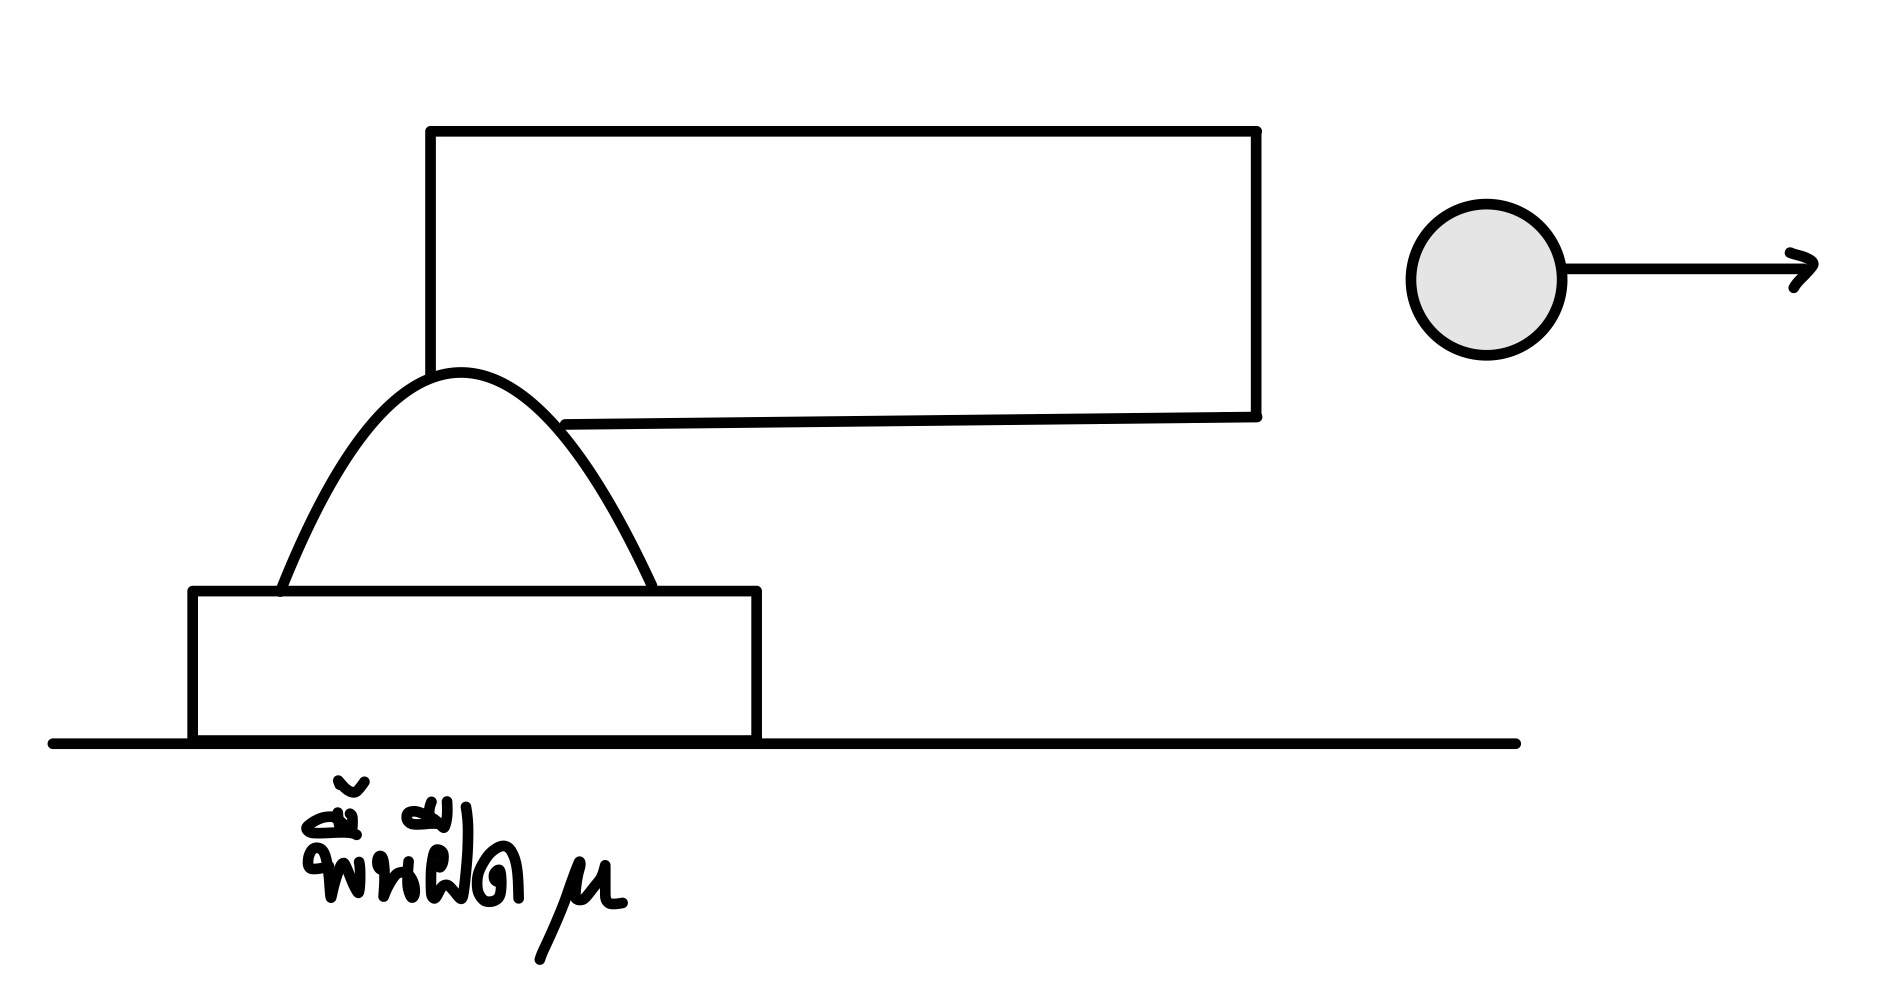
\includegraphics[width=0.5\linewidth]{26}
		\end{figure}
			\vspace{4cm}
		
		\item วางลูกบาศก์ A ยาวด้านละ \(\SI{1}{m}\) ลอยในน้ำที่มีความหนาแน่น \(\SI{1.0e3}{kg/m^3}\) จากนั้วางมวล B ทับมวล A ทำให้มวล A จมลงไป \(\SI{5.0}{cm}\) จงหาว่ามวล B มีค่ากี่\underline{กิโลกรัม}
		\begin{figure}[h]
			\centering
			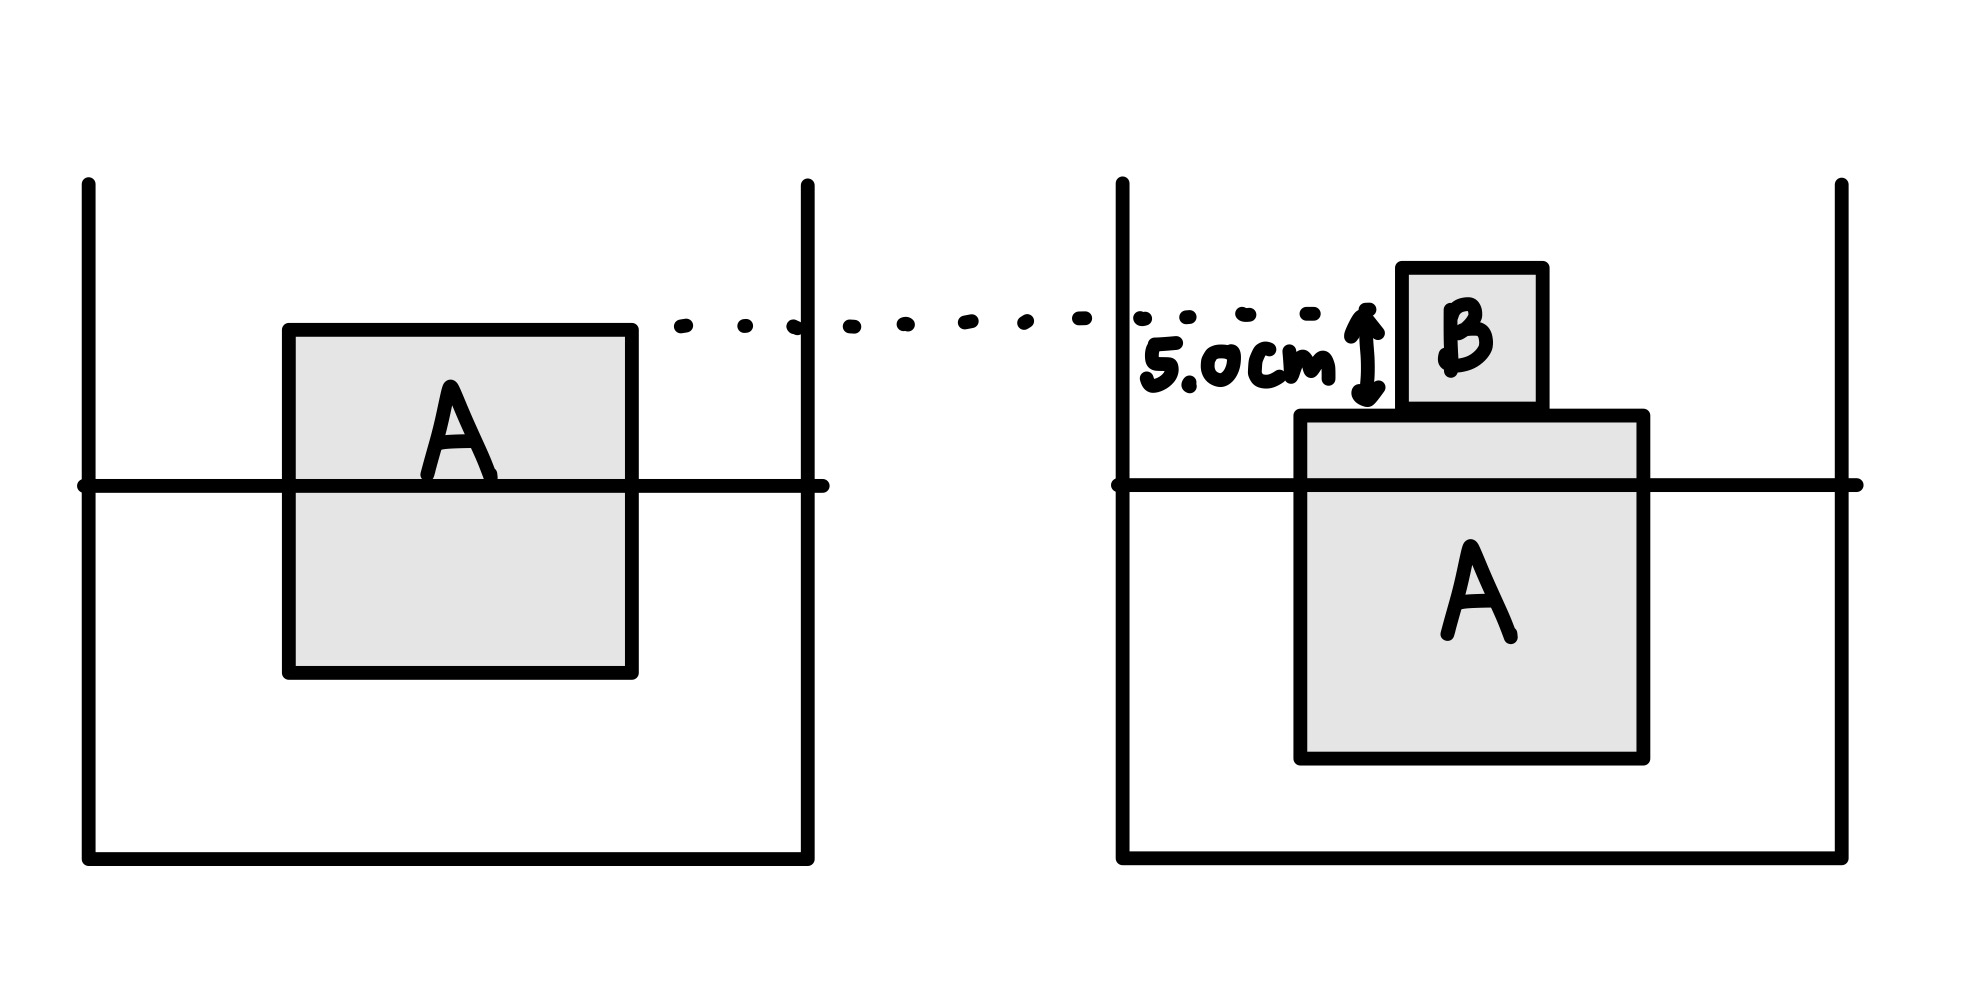
\includegraphics[width=0.5\linewidth]{27}
		\end{figure}
			\vspace{4cm}
		
		\item นักยิงธนู ต้องการยิงธนูเพื่อจุดคบเพลิงที่อยู่สูงจากพื้น \(\SI{21.6}{m}\) โดยยิงทำมุม \(\SI{45}{\degree}\) กับแนวระดับที่ความสูง \(\SI{2}{m}\) ดังภาพ
		ถ้าธนูใช้เวลาเคลื่อนที่ \(\SI{4}{s}\) จงหาว่าระยะระหว่างนักยิงธนูกับแท่นคบเพลิงในแนวระดับมีค่าเท่ากับกี่\underline{เมตร}
		\begin{figure}[h]
			\centering
			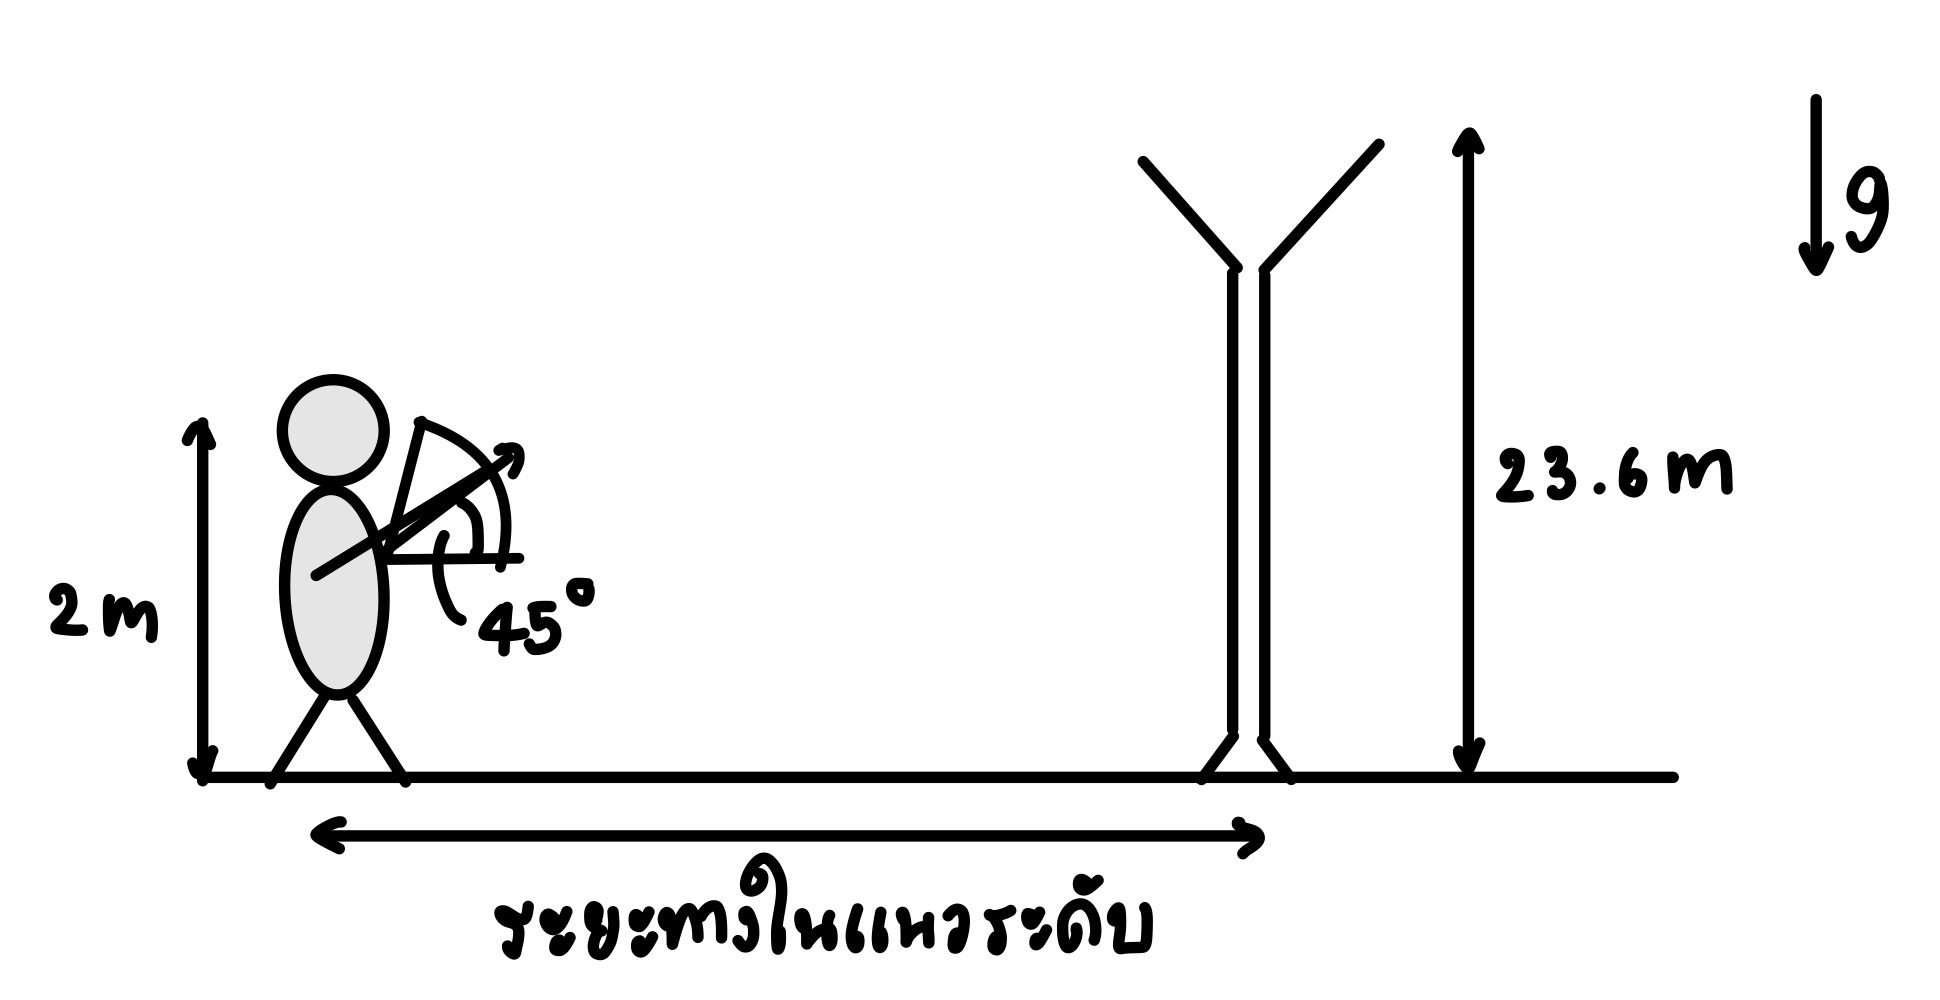
\includegraphics[width=0.5\linewidth]{28}
		\end{figure}
			\vspace{2cm}
		
		\item น้ำเคลื่อนที่ผ่านรอบต่อจากบริเวณน้ำลึก (บริเวณที่แรเงา\textenglish{)} ไปยังบริเวณน้ำตื้น โดยบริเวณน้ำลึกคลื่นเคลื่อนที่ด้วยอัตราเร็ว \(\sqrt{2}\,\si{m/s}\) จงหาว่าคลื่นจะเคลื่อนที่ผ่านบริเวณน้ำตื้นด้วยอัตราเร็วกี่\underline{เมตรต่อวินาที} (กำหนดให้ \(\sqrt{2}=1.41,\sqrt{3}=1.73\))
		\begin{figure}[h]
			\centering
			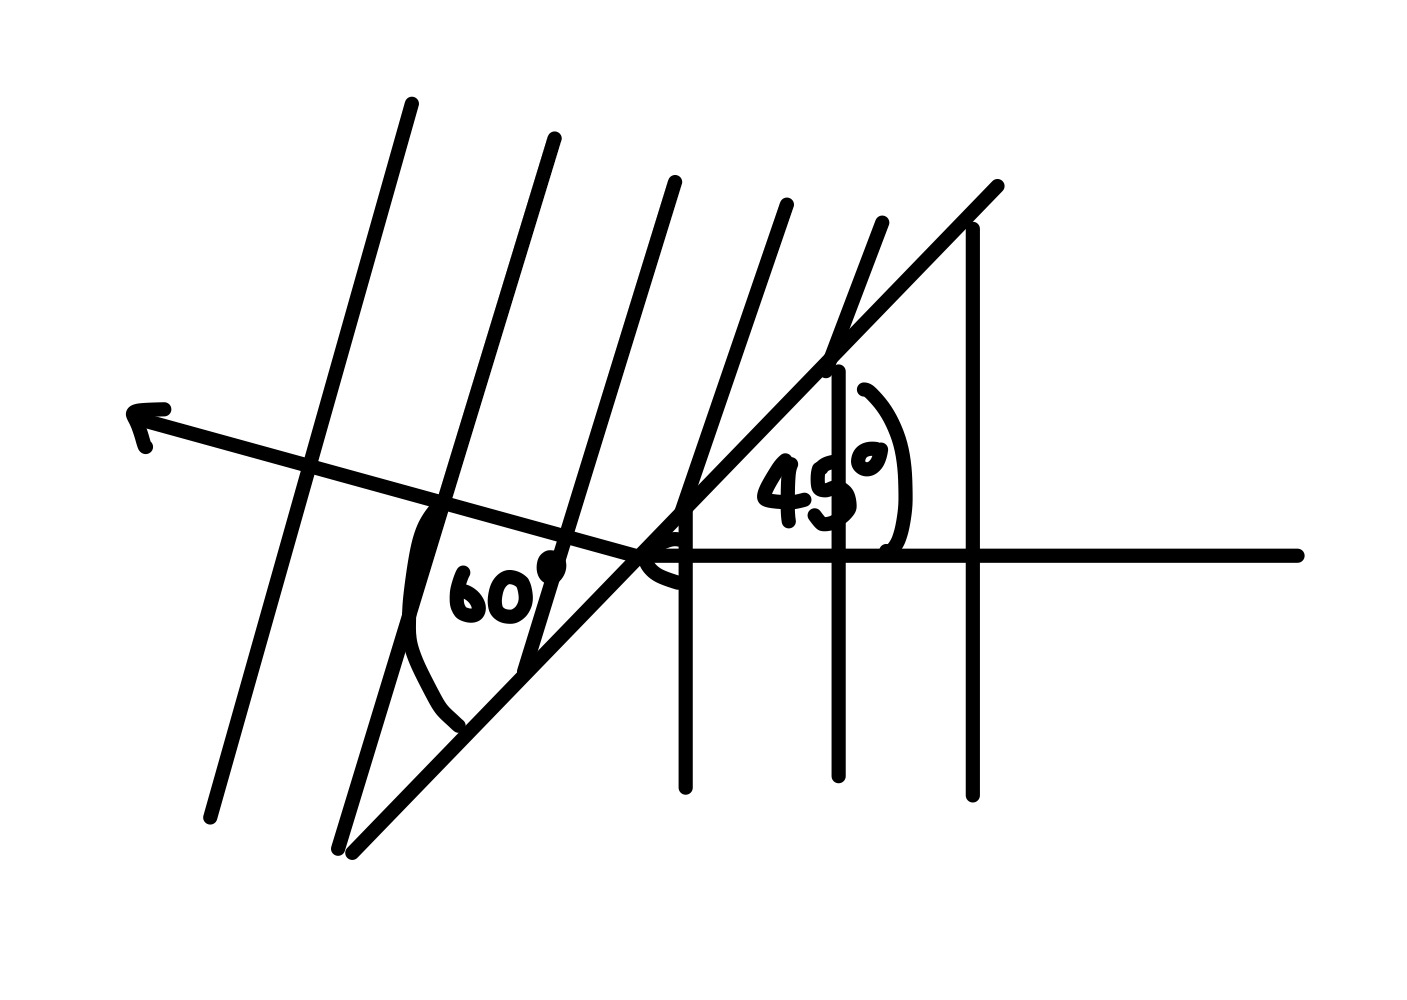
\includegraphics[width=0.3\linewidth]{29}
		\end{figure}
			\vspace{2cm}
		
		\item จงหากระแสไฟฟ้าที่ผ่านตัวต้านทาน \(\SI{2.4}{\ohm}\) ในหน่วย\underline{แอมแปร์}
		\begin{figure}[h]
			\centering
			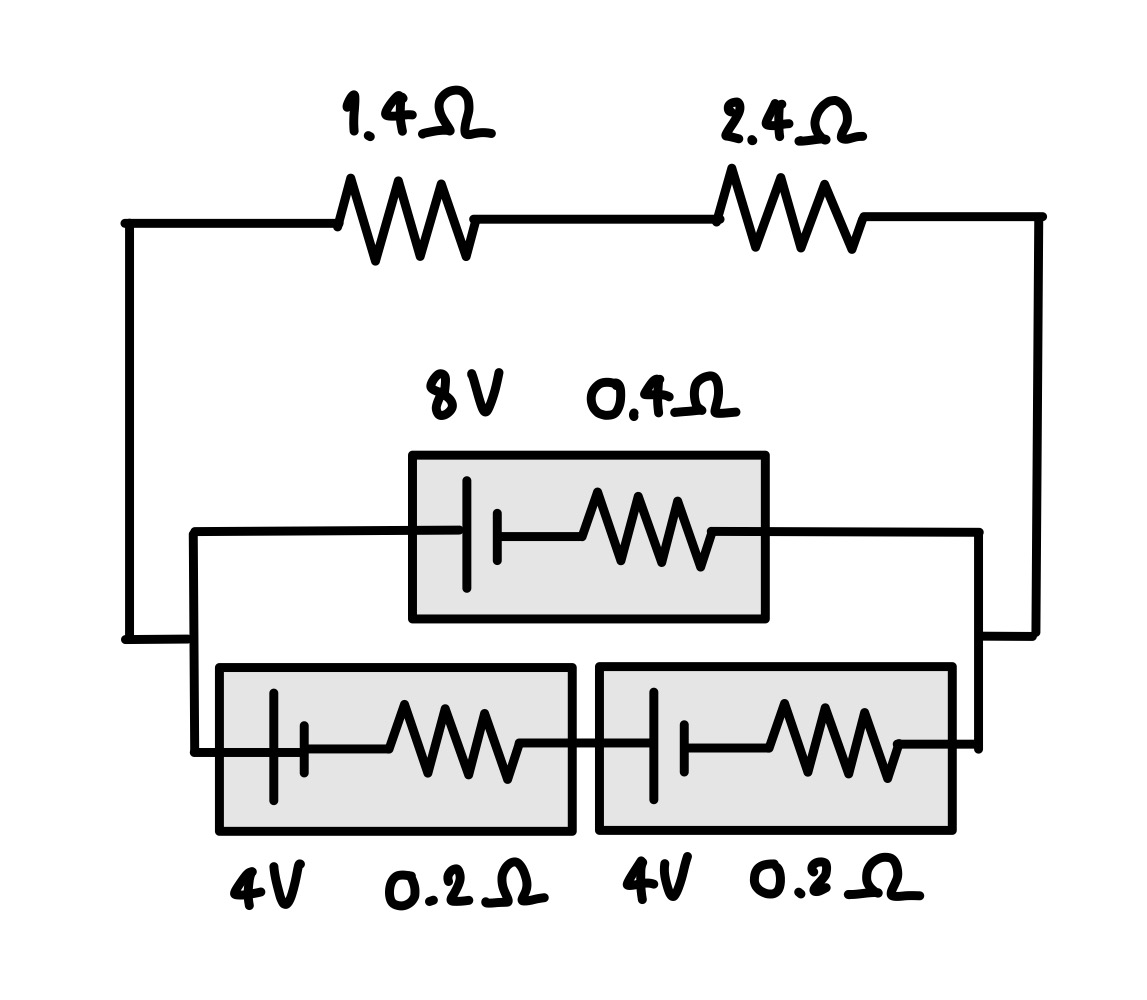
\includegraphics[width=0.3\linewidth]{30}
		\end{figure}
			\vspace{4cm}
\end{enumerate}
\newpage
\begin{center}
	\Large{เฉลย}
\end{center}
\begin{enumerate}
	\item 2
	\item กราฟผิดและโดนปรับ
	\item \(\SI{2}{m/s^2}\) ทำมุม \(\theta\) กับแกน \(-x\)
	\item \SI{11.8}{N}
	\item ขยับออก \SI{0.3}{m}
	\item \(\frac{W}{4}\)
	\item เท่ากัน
	\item \SI{2}{kg}
	\item ข และ ค
	\item \(4\pi\times10^{-5}\)
	\item \SI{1.00e-4}{m}
	\item \SI{6}{cm}
	\item \((1-\sqrt{2})\frac{kq}{d}\)
	\item \SI{24}{\micro J}
	\item ค
	\item 5
	\item 1
	\item 
	\item \(\SI{1250}{J/kg\cdot K}\) และ อุณหภูมิเท่าเดิม
	\item ข
	\item \(\dfrac{gL}{kA}\)
	\item \(2\sqrt{\dfrac{9P_0}{\rho}-gH}\)
	\item ข
	\item n=3 ไป n=2
	\item \SI{34.65}{s}
	\item \SI{9.8}{cm}
	\item \SI{50}{kg}
	\item \SI{100}{m}
	\item \SI{1}{m/s}
	\item \SI{2}{A}
\end{enumerate}
\end{document}